\documentclass[letterpaper,12pt]{article}

\usepackage{threeparttable}
\usepackage{geometry}
\geometry{letterpaper,tmargin=1in,bmargin=1in,lmargin=1.25in,rmargin=1.25in}
\usepackage[format=hang,font=normalsize,labelfont=bf]{caption}
\usepackage{amsmath}
\usepackage{multirow}
\usepackage{array}
\usepackage{delarray}
\usepackage{amssymb}
\usepackage{amsthm}
\usepackage{lscape}
\usepackage{natbib}
\usepackage{setspace}
\usepackage{float,color}
\usepackage[pdftex]{graphicx}
\usepackage{pdfsync}
\usepackage{verbatim}
\usepackage{placeins}
\usepackage{geometry}
\usepackage{pdflscape}
\synctex=1
\usepackage{hyperref}
\hypersetup{colorlinks,linkcolor=red,urlcolor=blue,citecolor=red}
\usepackage{bm}


\theoremstyle{definition}
\newtheorem{theorem}{Theorem}
\newtheorem{acknowledgement}[theorem]{Acknowledgement}
\newtheorem{algorithm}[theorem]{Algorithm}
\newtheorem{axiom}[theorem]{Axiom}
\newtheorem{case}[theorem]{Case}
\newtheorem{claim}[theorem]{Claim}
\newtheorem{conclusion}[theorem]{Conclusion}
\newtheorem{condition}[theorem]{Condition}
\newtheorem{conjecture}[theorem]{Conjecture}
\newtheorem{corollary}[theorem]{Corollary}
\newtheorem{criterion}[theorem]{Criterion}
\newtheorem{definition}{Definition} % Number definitions on their own
\newtheorem{derivation}{Derivation} % Number derivations on their own
\newtheorem{example}[theorem]{Example}
\newtheorem{exercise}[theorem]{Exercise}
\newtheorem{lemma}[theorem]{Lemma}
\newtheorem{notation}[theorem]{Notation}
\newtheorem{problem}[theorem]{Problem}
\newtheorem{proposition}{Proposition} % Number propositions on their own
\newtheorem{remark}[theorem]{Remark}
\newtheorem{solution}[theorem]{Solution}
\newtheorem{summary}[theorem]{Summary}
\bibliographystyle{aer}
\newcommand\ve{\varepsilon}
\renewcommand\theenumi{\roman{enumi}}
\newcommand\norm[1]{\left\lVert#1\right\rVert}

\begin{document}

\begin{titlepage}
\title{Integrating Microsimulation Tax Functions \\ into a DGE Macroeconomic Model: \\ A Canonical Example \thanks{This research benefited from support from the Brigham Young University Macroeconomics and Computational Laboratory and from the Open Source Policy Center at the American Enterprise Institute. All Python code and documentation for the computational model is available at \href{https://github.com/open-source-economics/OG-USA}{https://github.com/open-source-economics/OG-USA}.}
       }
       \author{
  Jason DeBacker\footnote{Middle Tennessee State University, Department of Economics and Finance, BAS N306, Murfreesboro, TN 37132, (615) 898-2528, \href{mailto:jason.debacker@mtsu.edu}{jason.debacker@mtsu.edu}.} \\[-2pt]
  \and
  Richard W. Evans\footnote{Brigham Young University, Department of Economics, 167 FOB, Provo, Utah 84602, (801) 422-8303, \href{mailto:revans@byu.edu}{revans@byu.edu}.} \\[-2pt]
  \and
  Kerk L. Phillips\footnote{Brigham Young University, Department of Economics, 166 FOB, Provo, Utah 84602, (801) 422-5928, \href{mailto:kerk_phillips@byu.edu}{kerk\_phillips@byu.edu}.}}
\date{March 2016}
\maketitle
\vspace{-9mm}
\begin{abstract}
\small{This paper integrates individual effective tax rate and marginal tax rate information from a microsimulation (partial equilibrium) model of tax policy with a dynamic scoring approach to tax policy analysis using a dynamic general equilibrium (DGE) macroeconomic model. Our approach integrates the rich heterogeneity, realistic demographics, and tax-code detail of the microsimulation model with the effects of tax changes on macroeconomic variables in the general equilibrium model. We use this approach to test the macroeconomic effects of the canonical example of a 10-percent cut in statutory marginal income tax rates. We find that such a tax cut increases GDP by about 1.6 percentage points in the long run.  Accounting for these effects of the tax change on GDP results in the an offset of about 40\% of the static cost of the tax cuts.
\vspace{3mm}

%\noindent\textit{keywords:}\: Static scoring, revenue estimates, dynamic scoring.
%
%\vspace{3mm}
%
%\noindent\textit{JEL classification:} (Put JEL codes here) C61, C63, D91, E21, H30, J11
}

\end{abstract}
\thispagestyle{empty}
\end{titlepage}


\begin{spacing}{1.5}

\section{Introduction}\label{SecIntro}

  In this paper, we describe the macroeconomics effects of a simple change in tax policy---a 10-percent reduction in all statutory marginal tax rates on personal income. For the purposes of our simulations, we assume these changes in tax law are permanent and are instituted on January 1, 2015 with no anticipatory effects.  This change is tax policy is a canonical example, used by \citet{CBO2004} and \citet{DM2011} to show the effects of various modeling approaches to dynamic analysis of tax policy.  Here, we use the same example to illustrate a novel approach to integrating a over-lappping generations model with a microsimulation model.

  Our approach to dynamic revenue estimation in this model is novel in that the tax functions we use in the general equilibrium macroeconomic model come directly from a microsimulation model for static revenue estimation. This allows us to integrate the rich heterogeneity, realistic demographics, and tax-code detail of the microsimulation model with the general equilibrium macroeconomic model. In addition, we have carefully calibrated the population demographics of the heterogeneous agents in our general equilibrium overlapping generations macroeconomic model.

  The paper is organized as follows. Section \ref{SecMicrosim} provides background on the microsimulation model we use to obtain the static revenue estimate. The DGE model we use to compute the macroeconomic changes is detailed in Section \ref{SecDGE}.  We describe our methodology for integrating the microsimulation and DGE models in Section \ref{SecIntegr}. We present some the results of the policy proposal example in Section \ref{SecResults}. Section \ref{SecDiscuss} provides a discussion of the qualitative results, along with the caveats and limitations of the model.


\section{Microsimulation Model: \texttt{Tax-Calculator}}\label{SecMicrosim}

  The microsimulation model we use is called \texttt{Tax-Caculator} and is developed and maintained by a group of researchers at the Open Source Policy Center (OSPC).\footnote{The documentation for using Tax-Calculator is available at \href{http://taxcalc.readthedocs.org/en/latest/index.html}{http://taxcalc.readthedocs.org/en/latest/index.html} A simple web application that provides an easy user interface for Tax-Calculator is available at \href{http://www.ospc.org/taxbrain/}{http://www.ospc.org/taxbrain/}. And all the source code is freely available at \href{https://github.com/open-source-economics/Tax-Calculator}{https://github.com/open-source-economics/Tax-Calculator}.} In this section, we outline the main structure of the \texttt{Tax-Calculator} microsimulation model, but encourage the interested reader to follow the links to the more detailed documentation.

  \texttt{Tax-Calculator} uses microdata on tax filers from the tax year 2009 Public Use Files (PUF) produced by the IRS. These data contain detailed records from the tax returns of about 200,000 tax filers who were selected from the population of filers through a stratified random sample of tax returns. These data come from IRS Form 1040 and a set of the associated forms and schedules. The PUF data are then matched to the Current Population Survey (CPS) to get imputed values for filer demographics such as age, which are not included in the PUF, and to incorporate households from the population of non-filers. The PUF-CPS match includes 219,815 filers.

  Since these data are for calendar year 2009, they must be ``aged" to be representative of the potential tax paying population in the years of interest (e.g. the current year through the end of the budget window).  To do this, macroeconomic forecasts of wages, interest rates, GDP, and other variables are used to grow the 2009 values to be representative of the values one might see in the years within the budget window. In addition to using macroeconomic variables to extrapolate the 2009 variables, a linear programming algorithm is used to re-weight the observations in each year in order to match target levels in the data such as total income and deduction amounts reported in more recent IRS data.

  Using these microdata, \texttt{Tax-Calculator} is able to determine total tax liability and marginal tax rates by computing each filer's tax reporting that minimizes the total tax liability subject to the parameters describing the tax policy. Our determination of total tax liability from the microsimulation model includes federal income taxes and payroll taxes but excludes state income taxes and estate taxes.\footnote{As the microsimulation model is further developed, we will account for these.} The output of the microsimulation model is forecasts of the total tax liability in each year derived from marginal tax rates, and items from the filers' tax returns for each of the 219,815 filers in the microdata. Population sampling weights are determined through the extrapolation and targeting of the microsimulation model. These weights allow one to calculate population representative results from the model. One can determine changes in tax liability and marginal tax rates by doing the same simulation where the parameters describing the tax policy are updated to reflect the proposed policy rather than the baseline policy. Note that the baseline policy is a current-law baseline.


\section{Dynamic General Equilibrium Model}\label{SecDGE}

  The DGE model in this paper is a close variant of the model used in \citet{DEMPRW2015}.\footnote{This paper can be downloaded at \href{http://mtweb.mtsu.edu/jdebacker/WealthTax.pdf}{http://mtweb.mtsu.edu/jdebacker/WealthTax.pdf}.} Our DGE model is comprised of heterogeneous individuals, perfectly competitive firms, and a government with a balanced budget requirement. A unit measure of identical firms make a static profit maximization decision in which they rent capital and hire labor to maximize profits given a Cobb-Douglas production function. The government levies taxes on individuals and makes lump sum transfers to individuals according to a balanced budget constraint. The model thus will present a relatively rich set of heterogeneity among households, but less in the production sector and a simple government sector.  Further development of the model along these other dimensions is ongoing. But the household sector is the most relevant to how we integrate these two models, even if other elements of the model such as government financing are important determinants of the macroeconomic outcomes.

  Individuals are assumed to live for a maximum of $E+S$ periods. We define an age-$s$ individual as being in youth and out of the workforce during ages $1\leq s\leq E$. We implement this dichotomy of being economically relevant by age in order to more easily match true population dynamics. Individuals enter the workforce at age $E+1$ and remain in the workforce until they die or until the maximum age $E+S$. Because of mortality risk, individuals can leave both intentional bequests at the end of life ($s=E+S$) as well as accidental bequests if they die before the maximum age of $E+S$.

  When individuals are born at age $s=1$, they are randomly assigned to one of $J$ lifetime earnings ability types. Individuals remain in their assigned lifetime earnings ability group throughout their lives. Once born and assigned to a group, an individual's lifetime earnings ability profile has a deterministic and known path. Related to hourly earnings, this process is calibrated to match the wage distribution by age in the United States, and labor is endogenously supplied by individuals. Our calibration of the hourly earnings process allows for a skewed distribution of earnings that fits U.S. life-cycle hourly earnings data. The economic environment is one of incomplete markets because the overlapping generations structure prevents households from perfectly smoothing consumption.


  \subsection{Population dynamics and lifetime earnings profiles}\label{SecPopDyn}

    One of the contributions of this paper is to carefully calibrate and incorporate population dynamics into dynamic revenue estimation. \citet{NishiyamaSmetters:2007} note that including realistic population dynamics in large-scale overlapping generations models has been restricted to a small number of studies.\footnote{\citet{DeNardiEtAl:1999}, \citet{KotlikoffEtAl:2001}, and \citet{Nishiyama:2004} include the effect of nonstationary demographics on macroeconomic variables.} Two likely reasons are the following. First, population dynamics introduce an additional source of growth to the model that must be stationarized in order to compute equilibrium solutions. And population demographics take a large number of years to reach their steady-state. This significantly increases the computation time for equilibrium solutions. A more detailed description of the population dynamics can be found in Appendix \ref{AppPopDyn}.

    We define $\omega_{s,t}$ as the number of individuals of age $s$ alive at time $t$. A measure $\omega_{1,t}$ of individuals with heterogeneous working ability is born in each period $t$ and live for up to $E+S$ periods, with $S\geq 4$.\footnote{Theoretically, the model works without loss of generality for $S\geq 3$. However, because we are calibrating the ages outside of the economy to be one-fourth of $S$ (e.g., ages 21 to 100 in the economy, and ages 1 to 20 outside of the economy), we need $S$ to be at least 4.} Individuals are termed ``youth'', and do not participate in market activity during ages $1\leq s\leq E$. The individuals enter the workforce and economy in period $E+1$ and remain in the workforce until they unexpectedly die or live until age $s=E+S$. We model the population with individuals age $s\leq E$ outside of the workforce and economy in order most closely match the empirical population dynamics.

    The population of agents of each age in each period $\omega_{s,t}$ evolves according to the following function,
    \begin{equation}\label{EqPopLawofmotion}
      \begin{split}
        \omega_{1,t+1} &= (1 - \rho_0)\sum_{s=1}^{E+S} f_s\omega_{s,t} + i_1\omega_{1,t}\quad\forall t \\
        \omega_{s+1,t+1} &= (1 - \rho_s)\omega_{s,t} + i_{s+1}\omega_{s+1,t}\quad\forall t\quad\text{and}\quad 1\leq s \leq E+S-1
      \end{split}
    \end{equation}
    where $f_s\geq 0$ is an age-specific fertility rate, $i_s$ is an age-specific net immigration rate, $\rho_s$ is an age specific mortality hazard rate,\footnote{The parameter $\rho_s$ is the probability that a individual of age $s$ dies before age $s+1$.} and $\rho_0$ is an infant mortality rate. The total population in the economy $N_t$ at any period is simply the sum of individuals in the economy, the population growth rate in any period $t$ from the previous period $t-1$ is $g_{n,t}$, $\tilde{N}_t$ is the working age population, and $\tilde{g}_{n,t}$ is the working age population growth rate in any period $t$ from the previous period $t-1$.
    \begin{equation}\label{EqPopN}
      N_t\equiv\sum_{s=1}^{E+S} \omega_{s,t} \quad\forall t
    \end{equation}
    \begin{equation}\label{EqPopGrowth}
      g_{n,t+1} \equiv \frac{N_{t+1}}{N_t} - 1 \quad\forall t
    \end{equation}
    \begin{equation}\label{EqPopNtil}
      \tilde{N}_t\equiv\sum_{s=E+1}^{E+S} \omega_{s,t} \quad\forall t
    \end{equation}
    \begin{equation}\label{EqPopGrowthTil}
      \tilde{g}_{n,t+1} \equiv \frac{\tilde{N}_{t+1}}{\tilde{N}_t} - 1 \quad\forall t
    \end{equation}

    At birth, a fraction $\lambda_j$ of the $\omega_{1,t}$ measure of new agents is randomly assigned to each of the $J$ lifetime income groups, indexed by $j=1,2,...J$, such that $\sum_{j=1}^J\lambda_j=1$. Note that lifetime income is endogenous in the model, therefore we define lifetime income groups by a particular path of earnings abilities. For each lifetime income group, the measure $\lambda_j\omega_{s,t}$ of individuals' effective labor units (which we also call ability) evolve deterministically according to $e_{j,s}$. This gives a different life cycle profile of earnings to each lifetime income group.  An individual's working ability evolves over its working-age lifetime $E+1\leq s \leq E+S$ according to this age-dependent deterministic process. The processes for the evolution of the population weights $\omega_{s,t}$ as well as lifetime earnings are exogenous inputs to the model.

    \begin{figure}[htb]\centering \captionsetup{width=4.0in}
      \caption{\label{FigLogAbility}\textbf{Exogenous life cycle income ability paths $\log(e_{j,s})$ with $S=80$ and $J=7$}}
      \fbox{\resizebox{4.0in}{2.7in}{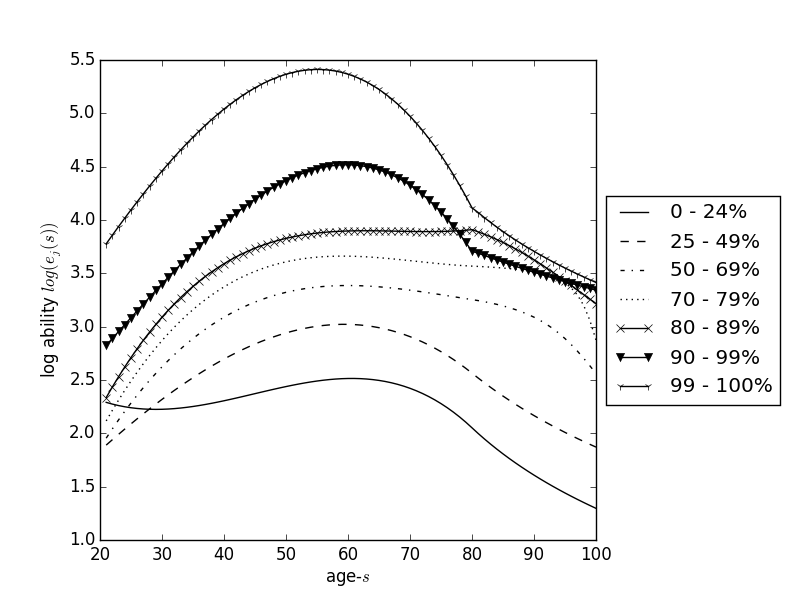
\includegraphics{./images/ability_log_2D_no_vline.png}}}
    \end{figure}

    Figure \ref{FigLogAbility} shows the calibrated trajectory of effective labor units (ability) $e_{j,s}\in\mathcal{E}\subset\mathbb{R}_{++}$ by age $s$ for each type $j$ for lifetime income distribution $\{\lambda_j\}_{j=1}^7 = [0.25,0.25,0.20,0.10,0.10,0.09,0.01]$. We show effective labor units in logarithms because the difference in levels between the top one percent and the rest of the distribution is so large. These exogenous earnings processes are taken from \citet{DEMPRW2015}.  All model individuals have the same time endowment and receive the same wage per effective labor unit, but some are endowed with more effective labor units. We utilize a measure of lifetime income, by using potential lifetime earnings, that allows us to define income groups in a way that accounts for the fact that earnings of individuals observed in the data are endogenous.  It is in this way that we are able to calibrate the exogenous lifetime earnings profiles form the model with their data counterparts.


  \subsection{Individual problem}\label{SecIndProb}

    Individuals are endowed with a measure of time $\tilde{l}$ in each period $t$, and they choose how much of that time to allocate between labor $n_{j,s,t}$ and leisure $l_{j,s,t}$ in each period. That is, an individual's labor and leisure choice is constrained by his total time endowment, which constraint is identical across all individuals.
    \begin{equation}\label{EqLabConstr}
      n_{j,s,t} + l_{j,s,t} = \tilde{l}
    \end{equation}
    At time $t$, all age-$s$ individuals with ability $e_{j,s}$ know the real wage rate, $w_t$, and know the one-period real net interest rate, $r_t$, on bond holdings, $b_{j,s,t}$, that mature at the beginning of period $t$. They also receive accidental and intentional bequests. They choose how much to consume $c_{j,s,t}$, how much to save for the next period by loaning capital to firms in the form of a one-period bond $b_{j,s+1,t+1}$, and how much to work $n_{j,s,t}$ in order to maximize expected lifetime utility of the following form,
    \begin{equation}\label{EqUtilMax}
      \begin{split}
        &U_{j,s,t} = \sum_{u=0}^{E+S-s}\beta^u\left[\prod_{v=s}^{s+u-1}(1-\rho_v)\right] u\left(c_{j,s+u,t+u},n_{j,s+u,t+u},b_{j,s+u+1,t+u+1}\right) \\
        &\text{and} \quad u\left(c_{j,s,t},n_{j,s,t},b_{j,s+1,t+1}\right) = \frac{\left(c_{j,s,t}\right)^{1-\sigma} - 1}{1-\sigma} ... \\
        &\qquad\qquad + e^{g_y t(1-\sigma)}\chi^n_s\left(b\left[1 - \left(\frac{n_{j,s,t}}{\tilde{l}}\right)^\upsilon\right]^\frac{1}{\upsilon} + k\right) + \rho_s\chi^b_j\frac{\left(b_{j,s+1,t+1}\right)^{1-\sigma} - 1}{1-\sigma} \\
        &\quad\quad\quad\quad\quad\quad\quad\quad\quad\quad\quad\quad\quad\quad\quad\quad\quad\quad\quad\forall j,t\quad\text{and}\:E+1\leq s\leq E+S
      \end{split}
    \end{equation}
    where $\sigma\geq 1$ is the coefficient of relative risk aversion on consumption and on intended (precautionary) bequests, $\beta\in(0,1)$ is the agent's discount factor, and the product term in brackets depreciates the individual's discount factor by the cumulative mortality rate. The disutility of labor term in the period utility function looks nonstandard, but is simply the upper right quadrant of an ellipse that closely approximates the standard CRRA utility of leisure functional form.\footnote{Appendix \ref{AppEllipseUtil} describes how the elliptical function closely matches the more standard constant Frisch elasticity disutility of labor of the form $-\frac{(n_{j,s,t})^{1+\theta}}{1+\theta}$. This elliptical utility function forces an interior solution that automatically respects both the upper and lower bound of labor supply, which greatly simplifies the computation of equilibrium. In addition, the elliptical disutility of labor has a Frisch elasticity that asymptotes to a constant rather than increasing to infinity as it does in the CRRA case. For a more in-depth discussion see \citet{EvansPhillips:2015}} The term $\chi^n_s$ is a constant term that varies by age $s$ influencing the disutility of labor relative to the other arguments in the period utility function,\footnote{\citet{DEMPRW2015} calibrate $\chi^n_s$ and $\chi^b_j$ to match average labor hours by age and some moments of the distribution of wealth.} and $g_y$ is a constant growth rate of labor augmenting technological progress, which we explain in Section \ref{SecFirms}.\footnote{The term with the growth rate $e^{g_y t(1-\sigma)}$ must be included in the period utility function because consumption and bequests will be growing at rate $g_y$ and this term stationarizes the individual Euler equation by making the marginal disutility of labor grow at the same rate as the marginal benefits of consumption and bequests.  This is the same balanced growth technique as that used in \citet{MertensRavn:2011}.}

    The last term in \eqref{EqUtilMax} incorporates a warm-glow bequest motive in which individuals value having savings to bequeath to the next generation in the chance they die before the next period. Including this term is essential to generating the positive wealth levels across the life cycle and across abilities that exist in the data. In addition, the term $\chi^b_j$ is a constant term that varies by lifetime income group $j$ influencing the marginal utility of bequests, $b_{j,s+1,t+1}$ relative to the other arguments in the period utility function. Allowing the $\chi^b_j$ scale parameter on the warm glow bequest motive vary by lifetime income group is critical for matching the distribution of wealth. As was mentioned in Section \ref{SecPopDyn}, individuals in the model have no income uncertainty because each lifetime earnings path $e_{j,s}$ deterministic, model agents thus hold no precautionary savings. Calibrating the $\chi^b_j$ for each income group $j$ captures in a reduced form way some of the characteristics that individual income risk provides.

    The parameter $\sigma\geq 1$ is the coefficient of relative risk aversion on bequests, and the mortality rate $\rho_s$ appropriately discounts the value of this term.\footnote{It is necessary for the coefficient of relative risk aversion $\sigma$ to be the same on both the utility of consumption and the utility of bequests. If not, the resulting Euler equations are not stationarizable.} Note that, because of this bequest motive, individuals in the last period of their lives ($s=S$) will die with positive savings $b>0$. Also note that the CRRA utility of bequests term prohibits negative wealth holdings in the model, but is not a strong restriction since none of the wealth data for the lifetime income group $j$ and age $s$ cohorts is negative except for the lowest quartile.

    The per-period budget constraints for each agent normalized by the price of consumption are the following,
    \begin{equation}\label{EqBC}
      \begin{split}
        &c_{j,s,t} + b_{j,s+1,t+1} \leq \left(1 + r_t\right) b_{j,s,t} + w_t e_{j,s}n_{j,s,t} + \frac{BQ_{j,t}}{\lambda_j\tilde{N}_t} - T_{s,t} \\
        &\qquad\qquad\qquad\text{where}\quad b_{j,E+1,t} = 0\quad\text{for} \quad E+1\leq s \leq E+S \quad \forall j,t
      \end{split}
    \end{equation}
    where $\tilde{N}_t$ is the total working age population at time $t$ defined in \eqref{EqPopNtil} and $\lambda_j\tilde{N}_t$ is the number of the total working individuals of type $j$ in period $t$. Note that the price of consumption is normalized to one, so $w_t$ is the real wage and $r_t$ is the net real interest rate. The term $BQ_{j,t}$ represents total bequests from individuals in income group $j$ who died at the end of period $t-1$. $T_{s,t}$ is a function representing net taxes paid, which we specify more fully below in equation \eqref{EqNetTaxLiab}.

    Implicit in the period budget constraint \eqref{EqBC} is a strong assumption about the distribution of bequests. We assume that bequests are distributed evenly across all ages to those in the same lifetime income group. It is difficult to precisely calibrate the distribution of bequests from the data, both across income types $j$ and across ages $s$. However, the assumptions about the bequest motive as well as how bequests are distributed are clearly important modeling decisions. Our current specification of bequests is the most persistent, which should make wealth inequality more persistent relative to other bequest specifications.\footnote{Another allocation rule at the opposite extreme would be to equally divide all bequests among all surviving individuals. An intermediate rule would be some kind of distribution of bequests with most going to ones own type and a declining proportion going to the other types.} A large number of papers study the effects of different bequest motives and specifications on the distribution of wealth, though there is no consensus regarding the true bequest transmission process.\footnote{See \citet{DeNardiYang:2014}, \citet{DeNardi:2004}, \citet{Nishiyama:2002}, \citet{Laitner:2001}, \citet{GokhaleEtAl:2001}, \citet{GaleScholz:1994}, \citet{Hurd:1989}, \citet{VentiWise:1988}, \citet{KotlikoffSummers:1981}, and \citet{Wolff:2015}.}

    Because the form of the period utility function in \eqref{EqUtilMax} ensures that $b_{j,s,t}>0$ for all $j$, $s$, and $t$, total bequests will always be positive $BQ_{j,t}>0$ for all $j$ and $t$.
    \begin{equation}\label{EqTotBeq}
      BQ_{j,t+1} = (1+r_{t+1})\lambda_j\left(\sum_{s=E+1}^{E+S}\rho_s\omega_{s,t}b_{j,s+1,t+1}\right) \quad\forall j,t
    \end{equation}
    In addition to each the budget constraint in each period, the utility function \eqref{EqUtilMax} imposes nonnegative consumption through infinite marginal utility, and the elliptical utility of leisure ensures individual labor and leisure must be strictly nonnegative $n_{j,s,t},l_{j,s,t}> 0$. Because individual savings or wealth is always strictly positive, the aggregate capital stock is always positive.\footnote{An alternative would be to allow for individual borrowing as long as an aggregate capital constraint $K_{t}>0$ for all $t$ is satisfied.} An interior solution to the individual's problem \eqref{EqUtilMax} is assured.

    In reality, each household is subject to many different taxes, all of which cannot be modeled in a DGE framework. It is the net tax liability function $T_{s,t}$ that we estimate from the microsimulation model output. This output includes information on all federal individual income and payroll taxes in the U.S. tax code. We also assume that every individual also receives an equal lump sum transfer $T^H_{t}$ which is generated from a balanced budget constraint on the government. Let $x$ represent stationary labor income, and let $y$ represent stationary capital income. We represent the net tax liability function as an effective tax rate times total labor and capital income.
    \begin{equation}\label{EqNetTaxLiab}
      \begin{split}
        T_{s,t}(x, y) &= \tau_{s,t}(x, y)\bigl(x + y\bigr) - T^H_t \\
        &\text{where}\quad x\equiv \frac{w_t e_{j,s}n_{j,s,t}}{e^{g_y t}} \quad\text{and}\quad y\equiv \frac{r_t b_{j,s,t}}{e^{g_y t}}
      \end{split}
    \end{equation}
    Note that the both the total tax liability function $T_{s,t}(x,y)$ and the effective tax rate functions $\tau_{s,t}(x,y)$ are functions of stationarized labor income $x$ and capital income $y$, separately. We detail the estimation of the tax functions $\tau_{s,t}(x,y)$ and $T_{s,t}(x,y)$ in Section \ref{SecIntegr}.

    The solution to the lifetime maximization problem \eqref{EqUtilMax} of individual with ability $j$ subject to the per-period budget constraint \eqref{EqBC} and the specification of taxes in \eqref{EqNetTaxLiab} is a system of $2S$ Euler equations. The $S$ static first order conditions for labor supply $n_{j,s,t}$ are the following,
    \begin{equation}\label{EqEulerLabGen}
      \begin{split}
        &(c_{j,s,t})^{-\sigma}\Biggl(w_t e_{j,s} - \frac{\partial T_{s,t}}{\partial n_{j,s,t}}\Biggr) = e^{g_y t(1-\sigma)}\chi^n_{s}\biggl(\frac{b}{\tilde{l}}\biggr)\biggl(\frac{n_{j,s,t}}{\tilde{l}}\biggr)^{v-1}\Biggl[1 - \biggl(\frac{n_{j,s,t}}{\tilde{l}}\biggr)^\upsilon\Biggr]^{\frac{1-v}{v}} \\
        &\qquad\qquad\qquad\qquad\qquad\qquad\qquad\qquad\qquad\forall j,t, \quad\text{and}\quad E+1\leq s\leq E+S \\
        &\qquad\text{where}\quad c_{j,s,t} = \left(1 + r_t\right) b_{j,s,t} + w_t e_{j,s}n_{j,s,t} + \frac{BQ_{j,t}}{\lambda_j\tilde{N}_t} - b_{j,s+1,t+1} - T_{s,t} \\
        &\qquad\text{and}\quad b_{j,E+1,t} = 0 \quad\forall j,t
      \end{split}
    \end{equation}
    where the marginal tax rate with respect to labor supply $\frac{\partial T_{s,t}}{\partial n_{j,s,t}}$ is described in equation \eqref{EqMTR_lab}.\footnote{We also have to use a parameter $factor$ that multiplies the model labor income and the model capital income in the tax function in order to match their levels to the corresponding average levels in the microsimulation model data. This is described in more detail in Section \ref{SecIntegrMicrosim}.}

    An individual also has $S-1$ dynamic Euler equations that govern his saving decisions, $b_{j,s+1,t+1}$, with the included precautionary bequest saving in case of unexpected death. These are given by:
    \begin{equation}\label{EqEulerSavGen}
      \begin{split}
        &(c_{j,s,t})^{-\sigma} = \rho_s\chi^b_j\bigl(b_{j,s+1,t+1}\bigr)^{-\sigma} + \beta(1-\rho_s)(c_{j,s+1,t+1})^{-\sigma}\Biggl[(1 + r_{t+1}) - \frac{\partial T_{s+1,t+1}}{\partial b_{j,s+1,t+1}}\Biggr] \\
        &\qquad\qquad\qquad\qquad\qquad\qquad\qquad\qquad\forall j,t,\quad\text{and}\quad E+1\leq s \leq E+S-1
      \end{split}
    \end{equation}
    where the marginal tax rate with respect to savings $\frac{\partial T_{s,t}}{\partial b_{j,s,t}}$ is described in equation \eqref{EqMTR_cap}. Lastly, Each individual also has one static first order condition for the last period of life $s=E+S$, which governs how much to bequeath to the following generation given that the individual will die with certainty. This condition is simply equation \eqref{EqEulerSavGen} with $\rho_s=1$.
    \begin{equation}\label{EqEulerSavEpS}
      (c_{j,E+S,t})^{-\sigma} = \chi^b_j(b_{j,E+S+1,t+1})^{-\sigma} \quad\forall j,t
    \end{equation}

    Define $\bm{\hat{\Gamma}}_t$ as the distribution of stationary individual savings across individuals at time $t$, including the intentional bequests of the oldest cohort.
    \begin{equation}\label{EqSavDist}
      \bm{\hat{\Gamma}}_t \equiv \Bigl\{\bigl\{\hat{b}_{j,s,t}\bigr\}_{j=1}^J\Bigr\}_{s=E+2}^{E+S+1} \quad\forall t
    \end{equation}
    As will be shown in Section \ref{SecMCEqlbm}, the state in every period $t$ for the entire equilibrium system described in the stationary, non-steady-state equilibrium characterized in Definition \ref{DefEquilNonSS} is the stationary distribution of individual savings $\bm{\hat{\Gamma}}_t$ from \eqref{EqSavDist}. Because individuals must forecast wages, interest rates, and aggregate bequests received in every period in order to solve their optimal decisions and because each of those future variables depends on the entire distribution of savings in the future, we must assume some individual beliefs about how the entire distribution will evolve over time. Let general beliefs about the future distribution of capital in period $t+u$ be characterized by the operator $\Omega(\cdot)$ such that:
    \begin{equation}\label{EqBeliefs}
      \bm{\hat{\Gamma}^e_{t+u}} = \Omega^u\left(\bm{\hat{\Gamma}_t}\right) \quad \forall t, \quad u\geq 1
    \end{equation}
    where the $e$ superscript signifies that $\hat{\Gamma}^e_{t+u}$ is the expected distribution of wealth at time $t+u$ based on general beliefs $\Omega(\cdot)$ that are not constrained to be correct.\footnote{In Section \ref{SecMCEqlbm} we will assume that beliefs are correct (rational expectations) for the stationary non-steady-state equilibrium in Definition \ref{DefEquilNonSS}.}


  \subsection{Firm problem}\label{SecFirms}

    A unit measure of identical, perfectly competitive firms exist in the economy. The representative firm is characterized by the following Cobb-Douglas production technology,
    \begin{equation}\label{EqCobbDougProd}
       Y_t = Z K_t^\alpha\left(e^{g_y t}L_t\right)^{1-\alpha} \quad \forall t
    \end{equation}
    where $Z$ is the measure of total factor productivity, $\alpha\in(0,1)$ is the capital share of income, $g_y$ is the constant growth rate of labor augmenting technological change, and $L_t$ is aggregate labor measured in efficiency units. The firm uses this technology to produce a homogeneous output which is consumed by individuals and used in firm investment.  The interest rate $r_t$ paid to the owners of capital is the real interest rate net of depreciation. The real wage is $w_t$.  The real profit function of the firm is the following.
    \begin{equation}\label{EqFirmProfit}
       \text{Real Profits} = Z K_t^\alpha\left(e^{g_y t}L_t\right)^{1-\alpha} - (r_t + \delta)K_t - w_t L_t
    \end{equation}
    As in the individual budget constraint \eqref{EqBC}, note that the price output has been normalized to one.

    Profit maximization results in the real wage, $w_t$, and the real rental rate of capital $r_t$ being determined by the marginal products of labor and capital, respectively:
    \begin{align}
       w_t &= (1-\alpha)\frac{Y_t}{L_t} \quad \forall t \label{EqFOCwage}\\
       r_t &= \alpha\frac{Y_t}{K_t} - \delta \quad\:\:\: \forall t \label{EqFOCrate}
    \end{align}


  \subsection{Government fiscal policy}\label{SecGovt}

    The government is represented by a balanced budget constraint. The government collects taxes $\tau_{s,t}(x,y)(x+y)$ from all individuals and divides total revenues equally among all economically active individuals in the economy to determine the lump-sum transfer.
    \begin{equation}\label{EqGovtBC}
      T^H_t = \frac{1}{\tilde N_t} \sum_s \sum_j \omega_{s,t}\lambda_j\tau_{s,t}(w_t e_{j,s}n_{j,s,t}, r_t b_{j,s,t})\bigl(w_t e_{j,s}n_{j,s,t} + r_t b_{j,s,t}\bigr)
    \end{equation}

    Lump sum transfers have an impact on the distribution of income and wealth. However, if one constrains policy experiments to have the same steady-state revenue impact, the changes in inequality in economic outcomes due to changes in government transfers is equivalent in each policy experiment in the steady-state.


  \subsection{Market clearing and stationary equilibrium}\label{SecMCEqlbm}

    Labor market clearing requires that aggregate labor demand $L_t$ measured in efficiency units equal the sum of individual efficiency labor supplied $e_{j,s}n_{j,s,t}$. Capital market clearing requires that aggregate capital demand $K_t$ equal the sum of capital investment by individuals $b_{j,s,t}$. Aggregate consumption $C_t$ is defined as the sum of all individual consumptions, and aggregate investment is defined by the resource constraint $Y_t = C_t + I_t$ as shown in \eqref{EqMktClrGoods}. That is, the following conditions must hold:
    \begin{align}
      L_t &= \sum_{s=E+1}^{E+S}\sum_{j=1}^{J} \omega_{s,t}\lambda_j e_{j,s}n_{j,s,t} \quad \forall t \label{EqMktClrLab} \\
      K_t &= \sum_{s=E+2}^{E+S+1}\sum_{j=1}^{J}\omega_{s-1,t-1}\lambda_j b_{j,s,t}  \quad \forall t \label{EqMktClrCap} \\
      \begin{split}
        Y_t &= C_t + K_{t+1} - (1-\delta)K_t \quad\forall t \\
        &\quad\text{where}\quad C_t \equiv \sum_{s=E+1}^{E+S}\sum_{j=1}^{J}\omega_{s,t}\lambda_j c_{j,s,t}
      \end{split} \label{EqMktClrGoods}
    \end{align}

    The usual definition of equilibrium would be allocations and prices such that individuals optimize \eqref{EqEulerLabGen}, \eqref{EqEulerSavGen}, and \eqref{EqEulerSavEpS}, firms optimize \eqref{EqFOCwage} and \eqref{EqFOCrate}, and markets clear \eqref{EqMktClrLab} and \eqref{EqMktClrCap}. However, the variables in the equations characterizing the equilibrium are potentially non-stationary due to the growth rate in the total population $g_{n,t}$ each period coming from the cohort growth rates in \eqref{EqPopLawofmotion} and from the deterministic growth rate of labor augmenting technological change $g_y$ in \eqref{EqCobbDougProd}.

    \begin{table}[htbp] \centering \captionsetup{width=3.3in}
    \caption{\label{TabStatVars}\textbf{Stationary variable definitions}}
      \begin{threeparttable}
      \begin{tabular}{>{\small}c >{\small}c >{\small}c |>{\small}c}
        \hline\hline
        \multicolumn{3}{c}{Sources of growth} & Not \\
        & & & \\[-4mm]
        $e^{g_y t}$ & $\tilde{N}_t$ & $e^{g_y t}\tilde{N}_t$ & growing\tnote{a} \\
        \hline
        & & \\[-4mm]
        $\hat{c}_{j,s,t}\equiv\frac{c_{j,s,t}}{e^{g_y t}}$ & $\hat{\omega}_{s,t}\equiv\frac{\omega_{s,t}}{\tilde{N}_t}$ & $\hat{Y}_t\equiv\frac{Y_t}{e^{g_y t}\tilde{N}_t}$ & $n_{j,s,t}$ \\[2mm]
        $\hat{b}_{j,s,t}\equiv\frac{b_{j,s,t}}{e^{g_y t}}$ & $\hat{L}_t\equiv\frac{L_t}{\tilde{N}_t}$ & $\hat{K}_t\equiv\frac{K_t}{e^{g_y t}\tilde{N}_t}$ & $r_t$ \\[2mm]
        $\hat{w}_t\equiv\frac{w_t}{e^{g_y t}}$ &  & $\hat{BQ}_{j,t}\equiv\frac{BQ_{j,t}}{e^{g_y t}\tilde{N}_t}$ &  \\[2mm]
        $\hat{y}_{j,s,t}\equiv\frac{y_{j,s,t}}{e^{g_y t}}$ &  & $\hat{C}_t\equiv \frac{C_t}{e^{g_y t}\tilde{N}_t}$  &  \\[2mm]
        $\hat{T}_{s,t}\equiv\frac{T_{j,s,t}}{e^{g_y t}}$ &  &  &  \\[2mm]
        \hline\hline
      \end{tabular}
      \begin{tablenotes}
        \scriptsize{\item[a]The interest rate $r_t$ in \eqref{EqFOCrate} is already stationary because $Y_t$ and $K_t$ grow at the same rate. Individual labor supply $n_{j,s,t}$ is stationary.}
      \end{tablenotes}
      \end{threeparttable}
    \end{table}

    Table \ref{TabStatVars} characterizes the stationary versions of the variables of the model in terms of the variables that grow because of labor augmenting technological change, population growth, both, or none. With the definitions in Table \ref{TabStatVars}, it can be shown that the equations  characterizing the equilibrium can be written in stationary form in the following way. The static and intertemporal first-order conditions from the individual's optimization problem corresponding to \eqref{EqEulerLabGen}, \eqref{EqEulerSavGen}, and \eqref{EqEulerSavEpS} are the following:

    \begin{equation}\label{EqEulerLabStat}
      \begin{split}
        &(\hat{c}_{j,s,t})^{-\sigma}\Biggl(\hat{w}_t e_{j,s} - \frac{\partial\hat{T}_{s,t}}{\partial n_{j,s,t}}\Biggr) = \chi^n_{s}\biggl(\frac{b}{\tilde{l}}\biggr)\biggl(\frac{n_{j,s,t}}{\tilde{l}}\biggr)^{\upsilon-1}\Biggl[1 - \biggl(\frac{n_{j,s,t}}{\tilde{l}}\biggr)^\upsilon\Biggr]^{\frac{1-\upsilon}{\upsilon}} \\
        &\qquad\qquad\qquad\qquad\qquad\qquad\qquad\qquad\forall j,t, \quad\text{and}\quad E+1\leq s\leq E+S \\
        &\qquad\text{where}\quad \hat{c}_{j,s,t} = \left(1 + r_t\right)\hat{b}_{j,s,t} + \hat{w}_t e_{j,s}n_{j,s,t} + \frac{\hat{BQ}_{j,t}}{\lambda_j} - e^{g_y}\hat{b}_{j,s+1,t+1} - \hat{T}_{s,t} \\
        &\qquad\text{and}\quad \hat{b}_{j,E+1,t} = 0 \quad\forall j,t
      \end{split}
    \end{equation}

    \begin{equation}\label{EqEulerSavStat}
      \begin{split}
        &(\hat{c}_{j,s,t})^{-\sigma} = ... \\
        &e^{-g_y\sigma}\Biggl(\rho_s\chi^b_j \bigl(\hat{b}_{j,s+1,t+1}\bigr)^{-\sigma} + \beta(1-\rho_s)(\hat{c}_{j,s+1,t+1})^{-\sigma}\Biggl[1 + r_{t+1} - \frac{\partial \hat{T}_{s+1,t+1}}{\partial \hat{b}_{j,s+1,t+1}}\Biggr]\Biggr) \\
        &\qquad\qquad\qquad\qquad\qquad\qquad\qquad\qquad\forall j,t,\quad\text{and}\quad E+1\leq s \leq E+S-1
      \end{split}
    \end{equation}

    \begin{equation}\label{EqEulerSavEpSstat}
      (\hat{c}_{j,E+S,t})^{-\sigma} = \chi^b_j e^{-g_y\sigma}(\hat{b}_{j,E+S+1,t+1})^{-\sigma} \quad\forall j,t
    \end{equation}

    The stationary firm first order conditions for optimal labor and capital demand corresponding to \eqref{EqFOCwage} and \eqref{EqFOCrate} are the following.
    \begin{equation}\label{EqFOCwageStat}
       \hat{w}_t = (1-\alpha)\frac{\hat{Y}_t}{\hat{L}_t} \quad \forall t
    \end{equation}
    \begin{equation}\tag{\ref{EqFOCrate}}
       r_t = \alpha\frac{\hat{Y}_t}{\hat{K}_t} - \delta = \alpha\frac{Y_t}{K_t} - \delta \quad \forall t
    \end{equation}
    And the two stationary market clearing conditions corresponding to \eqref{EqMktClrLab} and \eqref{EqMktClrCap}---with the goods market clearing by Walras' Law---are the following.
    \begin{align}
      \hat{L}_t &= \sum_{s=E+1}^{E+S}\sum_{j=1}^{J} \hat{\omega}_{s,t}\lambda_j e_{j,s}n_{j,s,t} \quad \forall t \label{EqMktClrLabStat} \\
      \hat{K}_t &= \frac{1}{1 + \tilde{g}_{n,t}}\left(\sum_{s=E+2}^{E+S+1}\sum_{j=1}^{J}\hat{\omega}_{s-1,t-1}\lambda_j \hat{b}_{j,s,t}\right) \quad \forall t \label{EqMktClrCapStat}
    \end{align}
    where $\tilde{g}_{n,t}$ is the growth rate in the working age population between periods $t-1$ and $t$ described in \eqref{EqPopGrowthTil}. The stationary version of the goods market clearing condition (aggregate resource constraint) is the following.
    \begin{equation}\label{EqMktClrGoodsStat}
      \hat{Y}_t = \hat{C}_t + e^{g_y}(1 + \tilde{g}_{n,t+1})\hat{K}_{t+1} - (1-\delta)\hat{K}_t \quad \forall t
    \end{equation}
    It is also important to note the stationary version of the characterization of total bequests $BQ_{j,t+1}$ from \eqref{EqTotBeq} and for the government budget constraint in \eqref{EqGovtBC}.
    \begin{equation}\label{EqTotBeqStat}
      \hat{BQ}_{j,t+1} = \frac{(1+r_{t+1})\lambda_j}{1+\tilde{g}_{n,t+1}}\left(\sum_{s=E+1}^{E+S}\rho_s\hat{\omega}_{s,t}\hat{b}_{j,s+1,t+1}\right) \quad\forall j,t
    \end{equation}
    \begin{equation}\label{EqGovtBCstat}
      \hat{T}^H_t = \sum_s \sum_j \hat{\omega}_{s,t}\lambda_j \hat{T}_{s,t}
    \end{equation}

    We can now define the stationary steady-state equilibrium for this economy in the following way.

    \vspace{7mm}
    \end{spacing}
    \hrule
    \begin{definition}[\textbf{Stationary steady-state equilibrium}]\label{DefEquilSS}
      A non-autarkic stationary steady-state equilibrium in the overlapping generations model with $S$-period lived agents and heterogeneous ability $e_{j,s}$ is defined as constant allocations $n_{j,s,t}=\bar{n}_{j,s}$ and $\hat{b}_{j,s+1,t+1}=\bar{b}_{j,s+1}$ and constant prices $\hat{w}_t=\bar{w}$ and $r_t=\bar{r}$ for all $j$, $s$, and $t$ such that the following conditions hold:
       \begin{enumerate}
          \item individuals optimize according to \eqref{EqEulerLabStat}, \eqref{EqEulerSavStat}, and \eqref{EqEulerSavEpSstat},
          \item Firms optimize according to \eqref{EqFOCwageStat} and \eqref{EqFOCrate},
          \item Markets clear according to \eqref{EqMktClrLabStat} and \eqref{EqMktClrCapStat}, and
          \item The population has reached its stationary steady state distribution $\bar{\omega}_s$ for all ages $s$, characterized in Appendix \ref{AppPopDyn}.
       \end{enumerate}
    \end{definition}
    \hrule
    \begin{spacing}{1.5}
    \vspace{10mm}

    The steady-state equilibrium is characterized by the system of $2JS$ equations and $2JS$ unknowns $\bar{n}_{j,s}$ and $\bar{b}_{j,s+1}$. Appendix \ref{AppSSsolve} details how to solve for the steady-state equilibrium.

    The non-steady state equilibrium is characterized by $2JST$ equations and $2JST$ unknowns, where $T$ is the number of periods along the transition path from the current state to the steady state.  The definition of the stationary non-steady-state equilibrium is similar to Definition \ref{DefEquilSS}, with the stationary steady-state equilibrium definition being a special case of the stationary non-steady-state equilibrium.

    \vspace{7mm}

    \hrule
    \begin{definition}[\textbf{Stationary non-steady-state equilibrium}]\label{DefEquilNonSS}
      A non-autarkic stationary non-steady-state equilibrium in the overlapping generations model with $S$-period lived agents and heterogeneous ability $e_{j,s}$ is defined as allocations $n_{j,s,t}$ and $\hat{b}_{j,s+1,t+1}$ and prices $\hat{w}_t$ and $r_t$ for all $j$, $s$, and $t$ such that the following conditions hold:
       \begin{enumerate}
          \item individuals have symmetric beliefs $\Omega(\cdot)$ about the evolution of the distribution of savings, and those beliefs about the future distribution of savings equal the realized outcome (rational expectations),
            \begin{equation*}
              \bm{\hat{\Gamma}}_{t+u} = \bm{\hat{\Gamma}}^e_{t+u} = \Omega^u\left( \bm{\hat{\Gamma}}_t\right) \quad\forall t, \quad u\geq 1
            \end{equation*}
          \item individuals optimize according to \eqref{EqEulerLabStat}, \eqref{EqEulerSavStat}, and \eqref{EqEulerSavEpSstat}
          \item Firms optimize according to \eqref{EqFOCwageStat} and \eqref{EqFOCrate}, and
          \item Markets clear according to \eqref{EqMktClrLabStat} and \eqref{EqMktClrCapStat}.
       \end{enumerate}
    \end{definition}
    \hrule

    \vspace{10mm}

    We describe the methodology to compute the solution to the non-steady-state equilibrium to Appendix \ref{AppNonSSsolve}.  We use the equilibrium transition path solution to find effects of tax policies on macroeconomic variables over the budget window.


  \subsection{Calibration}\label{SecCalib}

    Table \ref{TabExogVars} shows the calibrated values for the exogenous variables and parameters taken from \citet{DEMPRW2015}.

    \begin{table}[htbp] \centering \captionsetup{width=4.7in}
    \caption{\label{TabExogVars}\textbf{List of exogenous variables and baseline calibration values}}
      \begin{threeparttable}
      \begin{tabular}{>{\footnotesize}c |>{\footnotesize}l |>{\footnotesize}c}
        \hline\hline
        Symbol & \quad\quad\quad\quad Description & Value \\
        \hline
        $\bm{\hat{\Gamma}}_1$ & Initial distribution of savings & $\bm{\bar{\Gamma}}$ \\
        $N_0$ & Initial population & 1 \\
        $\{\omega_{s,0}\}_{s=1}^S$ & Initial population by age & (see App. \ref{AppPopDyn}) \\
        $\{f_s\}_{s=1}^S$ & Fertility rates by age & (see App. \ref{AppPopDyn}) \\
        $\{i_s\}_{s=1}^S$ & Immigration rates by age & (see App. \ref{AppPopDyn}) \\
        $\{\rho_s\}_{s=1}^S$ & Mortality rates by age & (see App. \ref{AppPopDyn}) \\
        $\{e_{j,s}\}_{j,s=1}^{J,S}$ & Deterministic ability process & (see \citealp{DEMPRW2015}) \\
        $\{\lambda_j\}_{j=1}^J$ & Lifetime income group percentages & $[0.25,0.25,0.20,0.10,0.10,0.09,0.01]$ \\
        $J$ & Number of lifetime income groups & 7 \\
        $S$ & Maximum periods in economically active & 80 \\[-2mm]
        &\quad individual life & \\
        $E$ & Number of periods of youth economically & $\text{round}\left(\frac{S}{4}\right)=20$ \\[-2mm]
        & \quad outside the model & \\
        $R$ & Retirement age (period) & $E+\text{round}\left(\frac{9}{16}S\right)=65$ \\
        \hline
        $\tilde{l}$ & Maximum hours of labor supply & 1 \\
        $\beta$ & Discount factor & $(0.96)^\frac{80}{S}$ \\
        $\sigma$ & Coefficient of constant relative risk aversion & 1.5 \\
        $b$ & Scale parameter in utility of leisure & 0.573 \\
        $\upsilon$ & Shape parameter in utility of leisure & 2.856 \\
        $k$ & constant parameter in utility of leisure & 0.000 \\
        $\chi^n_s$ & Disutility of labor level parameters & [19.041, 76.623] \\
        $\chi^b_j$ & Utility of bequests level parameters &  $[9.264 \times 10^{-5}, 118,648]$ \\ %$1.0 \ \forall j$ \\
        \hline
        $Z$ & Level parameter in production function & 1.0 \\
        $\alpha$ & Capital share of income & 0.35 \\
        $\delta$ & Capital depreciation rate & $1-(1-0.05)^\frac{80}{S}=0.05$ \\
        $g_y$ & Growth rate of labor augmenting & $(1+0.03)^\frac{80}{S}-1 = 0.03$ \\[-2mm]
        & \quad technological progress & \\
        \hline
        $T$ & Number of periods to steady state & 160 \\
        $\nu$ & Dampening parameter for TPI & 0.4 \\
        \hline\hline
      \end{tabular}
      \end{threeparttable}
    \end{table}

    Note that the scale parameter $\chi^n_s$ takes on 80 values (one for each model age) that increase with age, representing an increasing disutility of labor that is not modeled anywhere else in the utility function. An hour of labor for an older person becomes more costly due to biological reasons related to aging. Such a parametrization helps to fit fact that hours worked decline much more sharply later in life than do hourly earnings.

    Heterogeneity in the scale parameter multiplying useful in having the model generate a distribution of wealth similar to that observed in the data.  Note that without such heterogeneity in this parameter, individuals at the high end of the earnings distribution in our model would not save as much as their real world counterparts given the deterministic earnings process in our model. They have no precautionary savings motive, only the warm-glow bequest motive for savings.  One can view the assumption of heterogeneous utility weights as not just variation in preference across households, but also as reflecting differences in family size, expectations of income growth, or other variations that are not explicitly modeled here.  We thus allow  $\{\chi^b_j\}_{j=1}^7$ to take on seven values, one for each lifetime income group.


\section{Integration of Microsimulation Model with DGE Model}\label{SecIntegr}

  The main contribution of this paper is how we integrate the tax functions from the \texttt{Tax-Calculator} microsimulation model from Section \ref{SecMicrosim} into the DGE framework of the overlapping generations macroeconomic model described in Section \ref{SecDGE}. The nature of DGE models is such that they cannot accomodate the degree of policy and heterogeneity richness that actually exists in the economy. The analytics would be intractable and the computational burden would be too high. It would be too hard to model various filing types, such as single, married filing jointly, married filing separately, and head of household. Finding household optimal solutions across their lifetime with different income brackets for different tax rates would be nearly impossible due to the nonconvex optimization problem created by these policies.

  In contrast, the \texttt{Tax-Calculator} microsimulation model is perfectly suited to calculate the total taxes paid, effective tax rates, and marginal tax rates for a population with richly defined demographic heterogeneity. \texttt{Tax-Calculator} incorporates all the household levers and income brackets in the household tax code. We fit smooth approximating tax functions to the rich heterogeniety of the \texttt{Tax-Calculator} microsimulation model. We then use those functions in our DGE macroeconomic model. In this way, we incorporate all the complexities of the actual tax code into our macroeconomic model, which macroeconomic model is limited with regard to how much heterogeneity can be explicitly represented.

  We interface between the microsimulation and DGE model through the tax function $T_{s,t}$ in the household budget constraint \eqref{EqBC}. In particular, \texttt{Tax-Calculator} will produce microdata that can be used to calibrate these functions in a way that is consistent with the tax law parameters entered into the microsimulation model. Note that our estimated net tax liability function will be an approximation of the true underlying tax structure, incentives, and behavior, but our estimated parameters will fit smooth functions to the microsimulation model data that can be entered into the DGE model.

  We begin our discussion of the integration by describing the functional form we use approximate the effective tax rate function. We then explain how these functional forms are estimated using data generated by the microsimulation model and provide some measures of the fit of the functional form under the baseline tax policies. We also discuss how the tax parameters affecting payroll taxes are linked between the microsimulation and DGE models.

  In our DGE model, we need functions to represent the effective tax rate and the total tax liability, which is present in the household budget constraint \eqref{EqBC}. But we also need functions to represent the marginal tax rates with respect to both labor income and capital income. These marginal tax rates are present in the Euler equations \eqref{EqEulerSavStat}, and \eqref{EqEulerSavEpSstat}. One way to obtain the marginal tax rate functions is to simply use the analytical derivatives of the total tax liability functions. However, \citet[p.3]{BrillViard:2011} provide a canonical example of how variation in marginal tax rates can be masked by perceived smoothness in effective tax rates.\footnote{In this example, a revenue-neutral tax change is made that keeps effective tax rates constant, but drastically changes marginal tax rates.} For this reason, we use \texttt{Tax-Calculator} to independently estimate smooth functions for both effective tax rates and for marginal tax rates.


  \subsection{Modeling microsimulation tax structure}\label{SecIntegrMicrosim}

    Figure \ref{FigMicroTaxData3D} shows a scatter plot of effective tax rates from the \texttt{Tax-Calculator} microsimulation model plotted as a function of labor income an capital income for all 43-year-olds in the year 2015. Labor and capital income are truncated at \$600,000 in order to more clearly see the shape of the data in spite of the long right tail of the income distribution. Although there is noise in the data, effective tax rates are generally increasing in both labor and capital income at a decreasing rate from some slightly negative level to an asymptote around 30 percent. This regular shape in effective tax rates is observed for all ages in all years of the budget window.

    \begin{figure}[htbp]\centering \captionsetup{width=4.0in}
      \caption{\label{FigMicroTaxData3D}\textbf{Scatter plot of effective tax rates, labor income, and capital income from microsimulation model: $t=2015$ and $s=43$}}
      \fbox{\resizebox{4.0in}{3.0in}{\includegraphics{./images/MicroTaxData3D.png}}}
    \end{figure}

    Because of the regularity in the shape of the effective tax rates, we choose to fit a smooth function to these data that matches this shape. Our functional form is a ratio of polynomials in labor and capital income. Important properties of this functional form are that it produces this negative exponential form and it allows for negative effective tax rates at low levels of income. Estimating these functions for every age and every budget-window year also allows us to capture more of the heterogeneity from the microsimulation model that cannot be explicitly incorporated into the DGE model. As an example, filing status is correlated with age. While we could have fit functions of total tax liability or marginal tax rates, fitting the effective tax rate function has the benefit that the effective tax rate is roughly bounded above by one and roughly bounded below by zero when the income concept used is total economic income.

    Let $x$ be total labor income $x\equiv wen$, and let $y$ be total capital income $y\equiv rb$. Also, let the labor income share of total income be $\phi\equiv\frac{x}{x+y}=\frac{wen}{rb + wen}$.  We then write our effective tax rate functions as follows:

    \begin{equation}\label{EqATR}
      \begin{split}
        \tau(x,y) = &\Phi\Lambda + K \\
        &\text{where}\quad \Phi \equiv \Bigl[\phi(max_x - min_x) + (1 - \phi)(max_y - min_y)\Bigr] \\
        &\text{and}\quad \Lambda \equiv \biggl(\frac{Ax^2 + By^2 + Cxy + Dx + Ey}{Ax^2 + By^2 + Cxy + Dx + Ey + F}\biggr) \\
        &\text{and}\quad K \equiv \phi min_x + (1 - \phi)min_y \\
        &\text{where}\quad A,B,C,D,E,F,max_x,max_y > 0 \\
        &\text{and}\quad max_x > min_x \quad\text{and}\quad max_y > min_y
      \end{split}
    \end{equation}

    This functional form with the ratio of polynomials $\Lambda = \frac{z}{z + k}$ is a nice structure because it is bounded between 0 and 1 for positive polynomial coefficients and positive labor and capital income. The $\Phi$ term adjusts the upper and lower bounds of the tax function between the $x=0$ and $y=0$ planes. This class of functions also seems to robustly fit the shape of the tax data. The parameter $max_x$ is the maximum effective tax rate and $min_x$ is the minimum effective tax rate for all labor income $x$ when capital income is zero $y=0$. Conversely, the parameter $max_y$ is the maximum effective tax rate and $min_y$ is the minimum effective tax rate for all capital income $y$ when labor income is zero $x=0$. The parameters in the $\Phi$ and $K$ term allow for some simple slope changes from labor income to capital income to better fit the data. These parameters are summarized in Table \ref{TabTaxParams}.

    \begin{table}[htbp] \centering \captionsetup{width=3.7in}
    \caption{\label{TabTaxParams}\textbf{Description of tax function $\tau(x,y)$ parameters}}
      \begin{threeparttable}
      \begin{tabular}{>{\footnotesize}c |>{\footnotesize}l }
        \hline\hline
        Symbol & \quad\quad\quad\quad Description  \\
        \hline
        $A$ & Coefficient on squared $x$ term in $\tau(\cdot)$  \\
        $B$ & Coefficient on squared $y$ term in $\tau(\cdot)$  \\
        $C$ & Coefficient on interaction term in $\tau(\cdot)$  \\
        $D$ & Coefficient on linear $x$ term in $\tau(\cdot)$  \\
        $E$ & Coefficient on linear $y$ term in $\tau(\cdot)$  \\
        $F$ & Constant term in $\tau(\cdot)$\\
        $max_x$ & Maximum ETR on labor income $x$ given $y=0$  \\
        $min_x$ & Minimum ETR on labor income $x$ given $y=0$ \\
        $max_y$ & Maximum ETR on capital income $y$ given $x=0$ \\
        $max_y$ & Minimum ETR on capital income $y$ given $x=0$ \\
        \hline\hline
      \end{tabular}
      % \begin{tablenotes}
      %   \scriptsize{\item[]Note: Maybe put sources here.}
      % \end{tablenotes}
      \end{threeparttable}
    \end{table}

    \noindent Figure \ref{FigMicroTaxEst3D} shows the estimated surface from a nonlinear least squares estimation of the 10 parameters in Table \ref{TabTaxParams} to the data of Figure \ref{FigMicroTaxData3D}. This function fits the data closely, and adjusts whenever any of the many policy levers in the actual tax code are changed.

    \begin{figure}[htbp]\centering \captionsetup{width=5.0in}
      \caption{\label{FigMicroTaxEst3D}\textbf{Fitted tax function $\tau(x,y)$ versus microsimulation data $\tau_i$: $t=2015$ and $s=43$}}
      \fbox{\resizebox{5.0in}{4.0in}{\includegraphics{./images/MicroTaxEst3D.png}}}
    \end{figure}

    The total tax liability function is simply the effective tax rate function times total income $\tau(x,y)(x+y)$.
    \begin{equation}\label{EqTotTaxLiab}
      T(x,y) \equiv \tau(x,y)\bigl(x + y\bigr) = \bigl(\Phi\Lambda + K\bigr)\bigl(x + y\bigr)
    \end{equation}
    As discussed in the introduction to this section, one could use the expression in \eqref{EqTotTaxLiab} to solve for the marginal tax rates with respect to both total labor income $x$ and total capital income $y$. However, deriving the marginal tax rate function in this way ties them directly to the parameterization of the effective tax rate function. As referenced in \citet[p. 3]{BrillViard:2011}, this may present issues if one were to consider policies that affect the effective tax rate, but not marginal tax rates and vice versa. Such policies would include changes in the standard deduction or personal exemption amounts. In these cases, one would want the parameters of the effective tax rate function to change in a different way than parameters describing the marginal tax rate function. Thus we estimate separate functions for the marginal tax rates on labor and capital income.

    Figure \ref{FigMTRxyData} shows the marginal tax rates of an extra unit of labor income $x$ in panel 1 and an extra unit of capital income in panel 2 from \texttt{Tax-Calculator}. These marginal tax rates are again plotted as functions of labor income $x$ and capital income $y$. They are computed in \texttt{Tax-Calculator} by increasing the respective income by one penny and computing how much the total tax liability changes.

    \begin{figure}[htbp]\centering \captionsetup{width=6.0in}
      \caption{\label{FigMTRxyData}\textbf{Marginal tax rates data from \texttt{Tax-Calculator} as functions of labor income and capital income: $t=2015$ and $s=43$}}
      \fbox{\resizebox{6.0in}{2.7in}{\includegraphics{./images/MTRxyData.png}}}
    \end{figure}

    These marginal tax rate data in Figure \ref{FigMTRxyData} have negative exponential shapes similar to that of the effective tax rate data from Figure \ref{FigMicroTaxData3D}. We independently estimate a marginal tax rate of labor income function and a marginal tax rate of capital income function using the parameters of the same functional form from \eqref{EqATR} to match the corresponding data from Figure \ref{FigMTRxyData}. The resulting marginal tax rate functions from the respective estimated parameters are shown in Figure \ref{FigMTRxyEst}, with the red dots being the data and the yellow surfaces the respective estimated tax functions.

    \begin{figure}[htbp]\centering \captionsetup{width=6.0in}
      \caption{\label{FigMTRxyEst}\textbf{Estimated marginal tax rate functions as functions of labor income and capital income: $t=2015$ and $s=43$}}
      \fbox{\resizebox{6.0in}{2.7in}{\includegraphics{./images/MTRxyEst.png}}}
    \end{figure}

    The functional forms for the marginal tax rate of labor income is shown in \eqref{EqMTR_lab}, and the functional form for the marginal tax rate of capital income is shown in \eqref{EqMTR_cap}.

    \begin{equation}\label{EqMTR_lab}
      \begin{split}
       \frac{\partial T}{\partial x} = &\Phi_x\Lambda_x + K_x \\
        &\text{where}\quad \Phi_x \equiv \Bigl[\phi(max_{x,x} - min_{x,x}) + (1 - \phi)(max_{x,y} - min_{x,y})\Bigr] \\
        &\text{and}\quad \Lambda_x \equiv \biggl(\frac{A_x x^2 + B_x y^2 + C_x xy + D_x x + E_x y}{A_x x^2 + B_x y^2 + C_x xy + D_x x + E_x y + F_x}\biggr) \\
        &\text{and}\quad K_x \equiv \phi min_{x,x} + (1 - \phi)min_{x,y} \\
        &\text{where}\quad A_x,B_x,C_x,D_x,E_x,F_x,max_{x,x},max_{x,y} > 0 \\
        &\text{and}\quad max_{x,x} > min_{x,x} \quad\text{and}\quad max_{x,y} > min_{x,y}
      \end{split}
    \end{equation}

    \begin{equation}\label{EqMTR_cap}
      \begin{split}
       \frac{\partial T}{\partial y} = &\Phi_y\Lambda_y + K_y \\
        &\text{where}\quad \Phi_y \equiv \Bigl[\phi(max_{y,x} - min_{y,x}) + (1 - \phi)(max_{y,y} - min_{y,y})\Bigr] \\
        &\text{and}\quad \Lambda_y \equiv \biggl(\frac{A_y x^2 + B_y y^2 + C_y xy + D_y x + E_y y}{A_y x^2 + B_y y^2 + C_y xy + D_y x + E_y y + F_y}\biggr) \\
        &\text{and}\quad K_y \equiv \phi min_{y,x} + (1 - \phi)min_{y,y} \\
        &\text{where}\quad A_y,B_y,C_y,D_y,E_y,F_y,max_{y,x},max_{y,y} > 0 \\
        &\text{and}\quad max_{y,x} > min_{y,x} \quad\text{and}\quad max_{y,y} > min_{y,y}
      \end{split}
    \end{equation}

    The constraints on the parameters ensure that the marginal tax rates are not decreasing in income. While this might limit the model's ability to evaluate regressive tax policies, such policies pose theoretical issues for the model solution anyway due the presence of non-convex budget sets.

    The tax functions above are specific to a given age and tax year.  Thus, effective and marginal tax rates in the DGE model vary across the age of the model household, the model year, and amounts of capital and labor income. In this way, these tax functions incorporate some of the variation in statutory rates, as well as heterogeneity in income items, deductions items, credits, filing unit structure, and so forth into the DGE model that cannot account for this degree of heterogeneity. The effect of such heterogeneity on tax burdens will affect the effective tax rate functions we fit to the output of the microsimulation model. For example, if filing units with a primary filer that is 65 years old and with total income of \$60,000 have a higher proportion of income from tax exempt interest than do filing units who also have \$60,000 in total income, but a primary filer who is 40 years old, then the tax functions will be able to account for these different portfolios by finding a lower effective tax rate for the older filing unit than that younger filing unit, for a given amount of total income.

    We discussed earlier the alternative option for obtaining marginal tax rate functions by simply taking the analytical derivative of the total tax liability function in \eqref{EqTotTaxLiab} with respect to labor income and capital income, respectively, using the estimated effective tax rate function from \eqref{EqATR}. Figure \ref{FigEstVderMTRxy} shows the implied marginal tax rate functions described in this paragraph (red dots) versus the independently estimated tax rate functions described in this section (yellow surfaces).

    \begin{figure}[htbp]\centering \captionsetup{width=6.0in}
      \caption{\label{FigEstVderMTRxy}\textbf{Implied marginal tax rate functions vs. estimated marginal tax rate functions: $t=2015$ and $s=43$}}
      \fbox{\resizebox{6.0in}{2.7in}{\includegraphics{./images/EstVderMTRxy.png}}}
    \end{figure}

    Note that for the marginal tax rate of labor income in panel 1, the implied function as the derivative of \eqref{EqTotTaxLiab} with respect to labor income (red dots) is everywhere below the independently estimated function \eqref{EqMTR_lab}. And we know that the independently estimated function is a better fit to the marginal tax rates from \texttt{Tax-Calculator}. The same is true of the implied marginal tax rates of capital income in panel 2, except that the implied marginal tax rates are everywhere above the independently estimated marginal tax rates. For these reasons, we feel that the independently estimated marginal tax rates, in conjunction with our estimated effective tax rates, give us the most accurate approximation of individual incentives and behavior.

    Because the tax rates are estimated as functions of actual income in the data, which income levels can be in the millions of dollars, we have to map our model income units to the data income units. To do this, we estimate a parameter $factor$ such that $factor$ times average steady-state model income equals average data income.
    \begin{equation}\label{EqIncFactor}
      factor\sum_s \sum_j \bar{\omega}_s\lambda_j\left(\bar{w}e_{j,s}\bar{n}_{j,s} + \bar{r}\bar{b}_{j,s}\right) = \left(\text{data avg. income}\right)
    \end{equation}
    This we estimate this parameter to be $factor=113,412$. To be fully precise, the income levels in the model $x$ and $y$ in effective tax rate function \eqref{EqATR}, marginal tax rate of labor income function \eqref{EqMTR_lab}, and marginal tax rate of capital income function \eqref{EqMTR_cap} must be multiplied by this factor.


  \subsection{Estimating tax functions}\label{SecEstTaxFunc}

    Tax functions of the form above are estimated with output from the microsimulation model. Sample of effective tax rates and marginal tax rates (age $s=43$, period $t=2015$) from the \texttt{Tax-Calculator} microsimulation model are shown in Figures \ref{FigMicroTaxData3D} and \ref{FigMTRxyData}. To map the output of the microsimulation model, which is based on income reported on tax returns, to the DGE model, where income is defined more broadly, we use the following definitions.

    To calculate the effective tax rates from the microsimulation model, we divided total tax liability by a measure of ``adjusted total income".  Adjusted total income is defined as total income (Form 1040, line 22) plus tax-exempt interest income, IRA distributions, pension income, and Social Security benefits (Form 1040, lines 8b, 15a, 16a, and 20a, respectively).

    We consider adjusted total income from the microsimulation model to be the counterpart of total income in the DGE model. Total income in the DGE model is the sum of capital and labor income. We define labor income as earned income, which is the sum of wages and salaries (Form 1040, line 7) and self-employment income (Form 1040 lines 12 and 18) from the microsimulation model output. Capital income is defined as a residual.\footnote{This is not an ideal definition of capital income, since it includes transfers between filers (e.g., alimony payments) and from the government (e.g., unemployment insurance), but we have chosen this definition for now in order to ensure that all of total income is classified as either capital or labor income. This accounting will be refined in the future.}

    To calculate marginal tax rates on any given income source, we add one cent to that income source for each individual in the micro-data and then use the tax calculator to calculate the change in tax liability.  The change in tax liability divided by the change in income (one cent) yields the marginal tax rate.  To get the marginal tax rate on composite income amounts (e.g., labor income that is the sum of wage and self-employment income), we take a weighted average that accounts for negative income amounts.  In particular, to we calculate the weighted average marginal tax rate on composite of $n$ income sources as:

    \begin{equation}
    MTR_{composite} = \frac{\sum_{i=1}^{n} MTR_{n}*abs(Income_n)}{\sum_{i=1}^{n} abs(Income_n)}
    \end{equation}

    When we look at the raw output from the microsimulation model, we find that there are several observations with extreme values for their effective tax rate. Since this is a ratio, such outliers are possible, for example when the denominator, adjusted total income, is very small. We omit such outliers by making the following restrictions on the raw output of the microsimulation model. First, we exclude observations with an effective tax rate greater than 1.5 times the highest statutory marginal tax rate.  Second, we exclude observations where the effective tax rate is less than the lowest statutory marginal tax rate on income minus the maximum phase-in rate for the Earned Income Tax Credit (EITC).  Third, we drop observations with marginal tax rates in excess of 99\% or below the negative of the highest EITC rate (i.e., -45\% under current law).  These exclusions limit the influence of those with extreme values for their marginal tax rate, which are few and usually results from the income of the filer being right at a kink in the tax schedule.  Finally, since total income cannot be negative in our DGE model, we drop observations from the microsimulation model where adjusted total income is less than \$5.\footnote{We choose \$5 rather than \$0 to provided additional assurance that small income values are not driving large ETRs.}

    With the output of the microsimulation model cleaned, we move to our estimation. We estimate a transformation of the tax functions in Equations \eqref{EqATR}, \eqref{EqMTR_cap}, and \eqref{EqMTR_cap}  separately for each tax year and each year of age of the primary filer. That is, we estimate $\tau_{s,t}(x,y)$, $\frac{\partial T}{\partial y}\left(x,y\right)_{s,t}$, and $\frac{\partial T}{\partial y}\left(x,y\right)_{s,t}$. We transform these functions so that the labor income $x$ and capital income $y$ variables in the polynomials are transformed to percent deviations from their respective means. This helps with the scale of the variables in the optimization routine. The transformed ETR and MTR functions are estimated using a constrained, weighted, non-linear least squares estimator.  The weighting in this estimator come from the CPS weights assigned to the filers in the microsimulation model.

    Let $\bm{\theta}_{s,t}=(A,B,C,D,E,F,max_x,min_x,max_y,min_y)$ be the vector of parameters of the tax function for a particular age of filers in a particular year. The estimate $\bm{\hat{\theta}}_{s,t}$ is the following,
    \begin{equation}\label{EqThetaWSSQ}
      \begin{split}
        \bm{\hat{\theta}}_{s,t} = \bm{\theta}_{s,t}:\quad &\min_{\bm{\theta}_{s,t}}\sum_{i=1}^{N} \Bigl[\tau_{i}-\tau\bigl(x_i,y_i|\bm{\theta}_{s,t}\bigr)\Bigr]^{2} w_i, \\
        &\qquad\text{subject to}\quad A, B, C, D, E, F, max_x, max_y > 0 \\
        &\qquad\text{and}\quad max_{x}\geq min_x \quad\text{and}\quad max_{y}\geq min_y
      \end{split}
    \end{equation}
    where $\tau_{i}$ is the effective tax rate for observation $i$ from the microsimulation output, $\tau(x_i,y_i|\bm{\theta}_{s,t})$ is the predicted average tax rate for individual $i$ with $x_{i}$ labor income and $y_{i}$ capital income given parameters $\bm{\theta}_{s,t}$, and $w_{i}$ is the CPS sampling weight of this observation. The number $N$ is the total number of observations from the microsimulation output for age $s$ and year $t$. Figure \ref{FigMicroTaxEst3D} shows the typical fit of an estimated tax function $\tau_{s,t}\bigl(x,y|\bm{\theta}_{s,t}\bigr)$ to the data. The data in Figure \ref{FigMicroTaxEst3D} are the same age $s=43$ and year $t=2015$ as the data Figure \ref{FigMicroTaxData3D}. The only difference is that we have truncated both labor income $x$ and capital income $y$ in Figure \ref{FigMicroTaxData3D} at \$1 million rather than \$500,000. The parameters of the marginal tax rate functions are estimated in the same manner, and their respective estimated functions are shown in Figure \ref{FigMTRxyEst}.

    We use the microsimulation model data to estimate $S\times T$ sets of the 10 tax function parameters listed in Table \ref{TabTaxParams} for the ETR function and the two MTR functions. The total number of years of microsimulation data for which we estimate tax functions corresponds to the budget window of our desired revenue estimates, which is usually $T=10$. Because the DGE model has a time horizon well beyond 10 years, we assume that the file year tax policy in year $T$ is continued indefinitely from the end of the budget window forward. In addition, the data provide very few observations of primary filers with ages greater than 80 years old. The DGE model allows individuals to live for up to 100 periods.  We apply the tax function estimates for 80 year-olds to those with model ages 80-100.


\section{A 10\% Reduction in Income Tax Rates}\label{SecResults}

  The policy change we consider is a reduction in the marginal statutory rates on individual filers ordinary income.  This is the same example used to illustrate the workings of overlapping generations models by \citet{CBO2004} and \citet{DM2011}.  The changes in tax policy are summaries in Table \ref{tab:rates}.


  % Table generated by Excel2LaTeX from sheet 'PolicyChanges'
  \begin{table}[htbp]
    \centering
    \caption{Statutory Marginal Rates Under the Baseline and Policy Change}
      \begin{tabular}{ccc}
      \hline
      \hline
      Bracket & Baseline & Policy \\
      \hline
      1     & 0.100 & 0.090 \\
      2     & 0.150 & 0.135 \\
      3     & 0.250 & 0.225 \\
      4     & 0.280 & 0.252 \\
      5     & 0.330 & 0.297 \\
      6     & 0.350 & 0.315 \\
      7     & 0.396 & 0.356 \\
      \hline
      \hline
      \end{tabular}%
    \label{tab:rates}%
  \end{table}%


  \subsection{The Static Revenue Effects}

    Using the web application for the Tax-Calculator at \href{www.ospc.org/TaxBrain}{www.ospc.org/TaxBrain}, we calculate the revenue effects of the proposal to reduce the statutory marginal tax rate by 10\% for each tax bracket.  The static revenue effects as displaying on the Tax Brain webpage are about -\$1.25 trillion over 10 years (2015-2024).


    \begin{figure}[htbp]\centering \captionsetup{width=5.0in}
      \caption{\label{TaxBrainScore}\textbf{Static Revenue Estimate from the Tax Calculator}}
      \fbox{\resizebox{6.0in}{3.5in}{\includegraphics{./images/GalePropsalScreenShot.png}}}
    \end{figure}

We use the tax calculator to find the new effective and marginal tax rates faced by each of the filers represented in the PUF-CPS match under the reform.  We use these data to fit tax functions over income by year and primary filer age.  As explained above the fitted functions are then used in our DGE model to analyze the effect of the reform on macroeconomic aggregates and prices.

  \subsection{The Macroeconomic Effects}

    Table \ref{tab:macro} displays the percentage changes in aggregate quantities and prices over the budget window and in the long-run steady state.  These are computed through the DGE model described above, using the estimated tax functions for the baseline and policy tax parameters.  The parameters of the estimated tax functions are given in Table \ref{tab:tax_params}.

    % Table generated by Excel2LaTeX from sheet 'ParameterEstimates_baseline'
    \begin{table}[htbp]
      \centering
      \caption{Tax Function Parameters}
        \begin{tabular}{lrr}
        \hline
        \hline
        Parameter & Baseline & Policy \\
        \hline
        A     & 3.10E-10 & 9.45E-11 \\
        B     & 2.26E-10 & 1.57E-10 \\
        C     & 6.37E-12 & 7.29E-12 \\
        D     & 3.45E-04 & 1.99E-04 \\
        E     & 1.54E-04 & 7.94E-05 \\
        F     & 29.0441 & 18.3836 \\
        max\_{x} & 0.2910 & 0.2835 \\
        min\_{x} & -0.0544 & -0.0487 \\
        max\_{y} & 0.3037 & 0.2987 \\
        min\_{y} & -0.0240 & -0.0199 \\
        \hline
        \hline
        \end{tabular}%
      \label{tab:tax_params}%
    \end{table}%


    % Table generated by Excel2LaTeX from sheet 'Macros'
    \begin{table}[htbp]
    \scriptsize
      \centering
      \caption{Macroeconomic Effects of the Policy Change (\% Change)}
        \begin{tabular}{lrrrrrrrrrrrrrr}
        \hline
        \hline
              & 2015  & 2016  & 2017  & 2018  & 2019  & 2020  & 2021  & 2022  & 2023  & 2024  &       & 2015-2024 &       & SS \\
        \hline
        GDP   & 1.64 & 1.59 & 1.58 & 1.57 & 1.56 & 1.56 & 1.56 & 1.56 & 1.56 & 1.55 &       & 1.57 &       & 1.55 \\
        Consumption & 1.68 & 1.67 & 1.68 & 1.67 & 1.67 & 1.67 & 1.68 & 1.64 & 1.64 & 1.58 &       & 1.66 &       & 1.33 \\
        Investment & 3.66 & 3.22 & 2.68 & 3.48 & 2.33 & 3.24 & 3.06 & 2.62 & 2.85 & 2.22 &       & 2.92 &       & 2.04 \\
        Hours Worked & 1.94 & 1.73 & 1.53 & 1.83 & 1.37 & 1.74 & 1.66 & 1.44 & 1.53 & 1.23 &       & 1.60 &       & 1.18 \\
              &       &       &       &       &       &       &       &       &       &       &       &       &       &  \\
        Avg. Wage & 0.19 & 0.29 & 0.37 & 0.27 & 0.46 & 0.32 & 0.36 & 0.45 & 0.41 & 0.52 &       & 0.36 &       & 0.36 \\
        Interest Rate & -0.61 & -0.93 & -1.19 & -0.86 & -1.43 & -0.99 & -1.13 & -1.39 & -1.28 & -1.62 &       & -1.15 &       & -1.23 \\
              &       &       &       &       &       &       &       &       &       &       &       &       &       &  \\
        Total Taxes & -2.73 & -2.83 & -2.69 & -2.88 & -2.57 & -2.78 & -2.81 & -2.55 & -2.72 & -2.23 &       & -2.68 &       & -2.20 \\
        \hline
        \hline
        \end{tabular}%
      \label{tab:macro}%
    \end{table}%


\section{Discussion}\label{SecDiscuss}

  Qualitatively, the results of the macro model are consistent with economic theory. The reduction in marginal tax rates increases the incentives to work and save. We subsequently see increases aggregate hours worked and investment. As a result, both GDP and consumption increase.  That the increases in the capital stock are larger than the increase in hours worked, means that the marginal product of capital falls, while the marginal product of labor rises. Given our assumption of a competitive production sector, this results in lower real interest rates and higher wages.

  Total tax revenue decreases due to the lower tax rates, but the increase in aggregate income that results from the additional investment and labor supply offset the revenue losses to some extent.  Consider that the static score suggests revenue losses on the order of 4\% of total tax revenue. These losses are between 2\% and 3\% when accounting for the macroeconomic effects of the tax policy.

  A few caveats about the limitations of the model are in order.  Of first order importance in determining the macroeconomic effects of changes in tax policy are the assumptions about how such tax changes are financed (see \citet{DM2011} for a comparison of results under different financing options).  The DGE model used here has a simple balanced budget requirement for the government. This means that tax cuts, as we consider here, are financed by immediate reductions in the lump sum transfers the government makes to all households. The assumption is the most conducive to reductions in taxes providing positive macroeconomic effects.  If these tax cuts were temporary and financed by future tax increases, the stimulative effects of such cuts would be substantially reduced.  In fact, our long run change in GDP of 1.6 percentage points, lies well above the upper bounds found by \citet{DM2011} and \citet{CBO2004}.  Such differences are largely driven by assumptions regarding how tax cuts are financed, but are also due to differences in model parameterizations and other features.

  Not considered in this model but also important in determining the macroeconomic effects of fiscal policy are the policy responses of the central bank.  Implicit in the results presented here is that the central bank does not respond to fiscal policy.  If, for example, the central bank responded by holding interest rates constant, the supply side effects would be smaller and their would be less of a change in the macroeconomic aggregates.

  Finally, one should note that while the levels of the macroeconomic aggregates change in the steady state as a result of tax policy, that long run growth rates do not.  These long run growth rates are governed by exogenous changes in population growth and factor productivity.  Thus these long run growth rates, in this framework, are not dependent on tax policy.





  \clearpage


\end{spacing}


\newpage
\bibliography{DEP_10pct}


\newpage
\renewcommand{\theequation}{A.\arabic{section}.\arabic{equation}}
                                                 % redefine the command that creates the section number
\renewcommand{\thesection}{A-\arabic{section}}   % redefine the command that creates the equation number
\setcounter{equation}{0}                         % reset counter
\setcounter{section}{0}                          % reset section number
\section*{APPENDIX}                              % use *-form to suppress numbering

\section{Characteristics of exogenous population dynamics}\label{AppPopDyn}

  In this appendix, we detail how we generate the exogenous population dynamics that are inputs to the model described in Section \ref{SecPopDyn}. All output, tests, functions, and computation in this chapter are available in the \href{https://github.com/rickecon/OG-USA/blob/demog/Python/ogusa/demog.py}{\texttt{demog.py}} file.

  \begin{figure}[htbp]\centering \captionsetup{width=4.0in}
    \caption{\label{FigPerTime}\textbf{Correspondence of model timing to data timing for model periods of one year}}
    \fbox{\resizebox{4.0in}{2.0in}{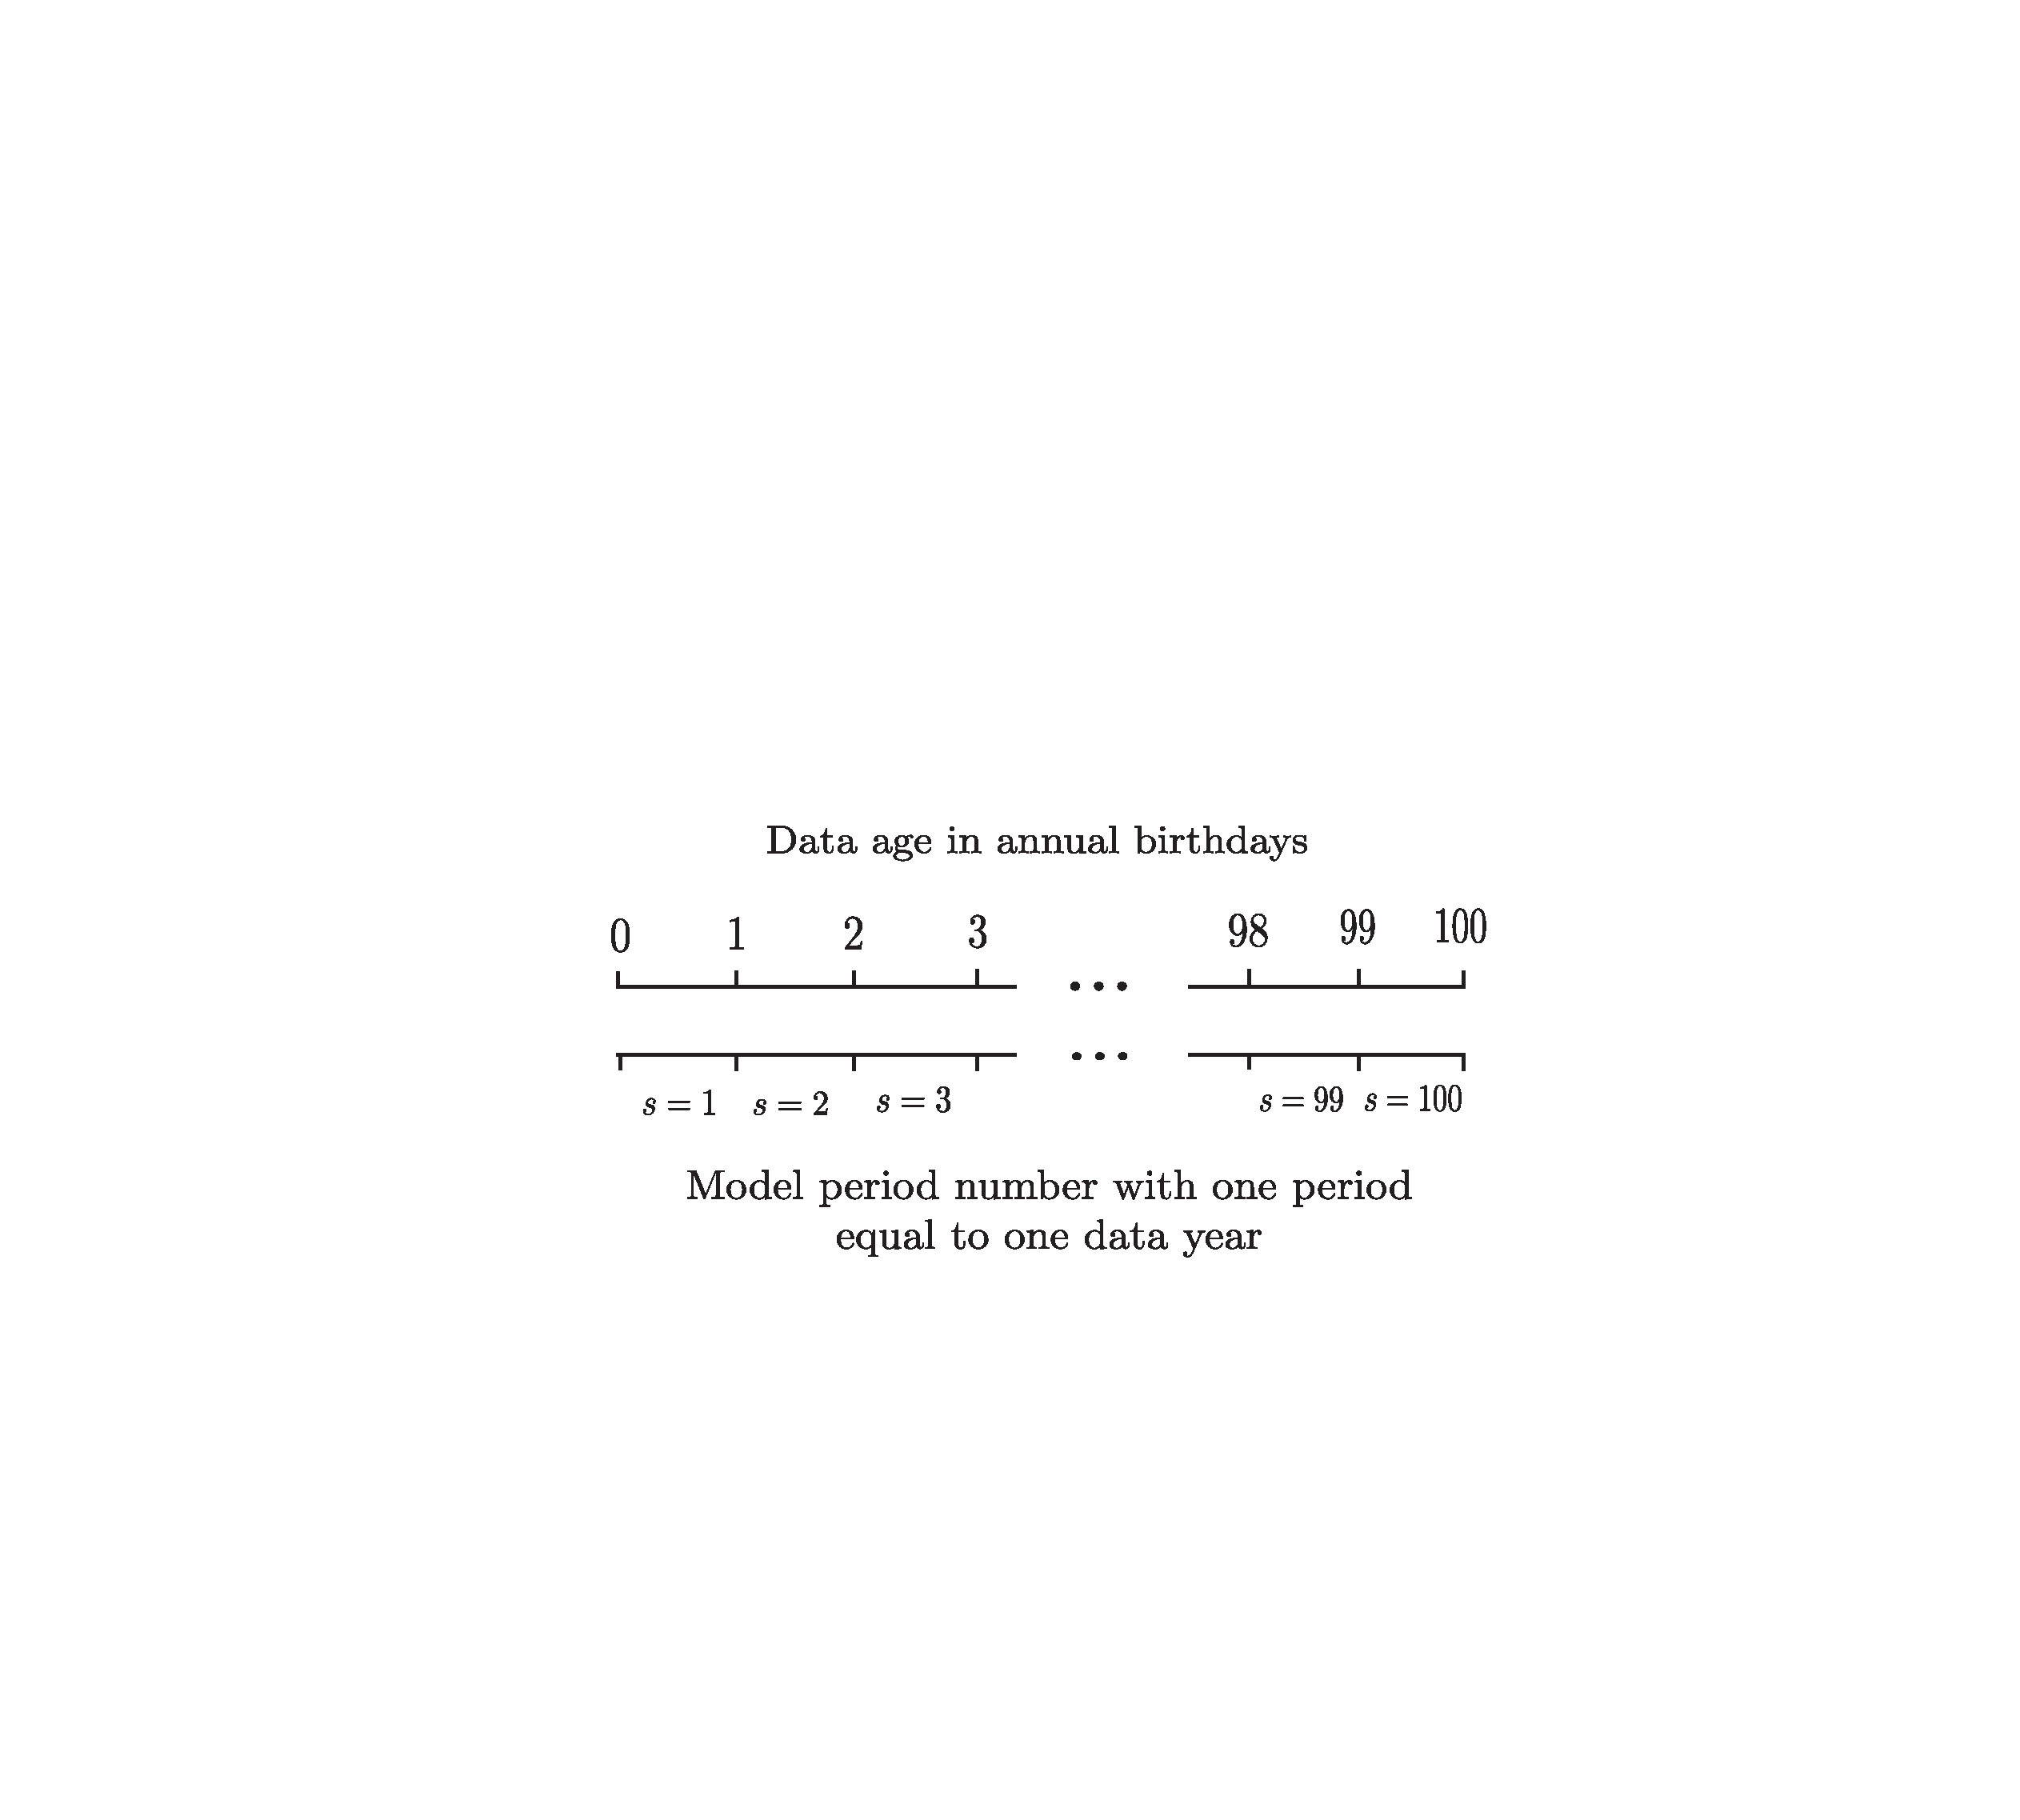
\includegraphics{./images/FigPerTime.pdf}}}
  \end{figure}

  Figure \ref{FigPerTime} shows the correspondence between model periods and data periods. Period $s=1$ corresponds to the first year of life between birth and when an individual turns one year old. We use this convention to match our model periods to those in the data.


  \subsection{Nonstationary and stationary population dynamics}\label{AppPopNonStatStat}

    We define $\omega_{s,t}$ as the number of individuals of age $s$ alive at time $t$. A measure $\omega_{1,t}$ of individuals with heterogeneous working ability is born in each period $t$ and live for up to $E+S$ periods, with $S\geq 4$.\footnote{Theoretically, the model works without loss of generality for $S\geq 3$. However, because we are calibrating the ages outside of the economy to be one-fourth of $S$ (e.g., ages 21 to 100 in the economy, and ages 1 to 20 outside of the economy), we need $S$ to be at least 4.} Individuals are termed ``youth'', and do not participate in market activity during ages $1\leq s\leq E$. The individuals enter the workforce and economy in period $E+1$ and remain in the workforce until they unexpectedly die or live until age $s=E+S$. We model the population with individuals age $s\leq E$ outside of the workforce and economy in order most closely match the empirical population dynamics.

    The population of agents of each age in each period $\omega_{s,t}$ evolves according to the following function,
    \begin{equation}\tag{\ref{EqPopLawofmotion}}
      \begin{split}
        \omega_{1,t+1} &= (1 - \rho_0)\sum_{s=1}^{E+S} f_s\omega_{s,t} + i_1\omega_{1,t}\quad\forall t \\
        \omega_{s+1,t+1} &= (1 - \rho_s)\omega_{s,t} + i_{s+1}\omega_{s+1,t}\quad\forall t\quad\text{and}\quad 1\leq s \leq E+S-1
      \end{split}
    \end{equation}
    where $f_s\geq 0$ is an age-specific fertility rate, $i_s$ is an age-specific net immigration rate, $\rho_s$ is an age specific mortality hazard rate,\footnote{The parameter $\rho_s$ is the probability that a individual of age $s$ dies before age $s+1$.} and $\rho_0$ is an infant mortality rate. The total population in the economy $N_t$ at any period is simply the sum of individuals in the economy, the population growth rate in any period $t$ from the previous period $t-1$ is $g_{n,t}$, $\tilde{N}_t$ is the working age population, and $\tilde{g}_{n,t}$ is the working age population growth rate in any period $t$ from the previous period $t-1$.
    \begin{equation}\tag{\ref{EqPopN}}
      N_t\equiv\sum_{s=1}^{E+S} \omega_{s,t} \quad\forall t
    \end{equation}
    \begin{equation}\tag{\ref{EqPopGrowth}}
      g_{n,t+1} \equiv \frac{N_{t+1}}{N_t} - 1 \quad\forall t
    \end{equation}
    \begin{equation}\tag{\ref{EqPopNtil}}
      \tilde{N}_t\equiv\sum_{s=E+1}^{E+S} \omega_{s,t} \quad\forall t
    \end{equation}
    \begin{equation}\tag{\ref{EqPopGrowthTil}}
      \tilde{g}_{n,t+1} \equiv \frac{\tilde{N}_{t+1}}{\tilde{N}_t} - 1 \quad\forall t
    \end{equation}

    We can transform the nonstationary equations in \eqref{EqPopLawofmotion} into stationary laws of motion by dividing both sides by the total economically relevant population in the current period $\tilde{N}_t$ and then multiplying the left-hand-side of the equation by $\tilde{N}_{t+1}/\tilde{N}_{t+1}$,
    \begin{equation}\label{EqPopLawofmotionStat}
      \begin{split}
        \hat{\omega}_{1,t+1} &= \frac{(1-\rho_0)\sum_{s=1}^{E+S} f_s\hat{\omega}_{s,t} + i_1\hat{\omega}_{1,t}}{1+\tilde{g}_{n,t+1}}\quad\forall t \\
        \hat{\omega}_{s+1,t+1} &= \frac{(1 - \rho_s)\hat{\omega}_{s,t} + i_{s+1}\hat{\omega}_{s+1,t}}{1+\tilde{g}_{n,t+1}}\qquad\quad\:\forall t\quad\text{and}\quad 1\leq s \leq E+S-1
      \end{split}
    \end{equation}
    where $\hat{\omega}_{s,t}$ is the percent of the total economically relevant population $\tilde{N}_t$ in age cohort $s$ in period $t$, and $\tilde{g}_{n,t+1}$ is the population growth rate between periods $t$ and $t+1$ defined in \eqref{EqPopGrowthTil}.\footnote{Note in the specification of the stationary laws of motion \eqref{EqPopLawofmotionStat} that $\sum_{s=1}^{E+S}\hat{\omega}_{s,t}>1$ while $\sum_{s=E+1}^{E+S}\hat{\omega}_{s,t}=1$. This is because in the model we only look at the economically relevant population $\hat{\omega}_{s,t}$ for $E+1\leq s\leq E+S$.}


  \subsection{Fertility Rates}\label{AppPopFert}

    In this model, we assume that the fertility rates for each age cohort $f_s$ are constant across time. However, this assumption is conceptually straightforward to relax. Our data for U.S. fertility rates by age come from \citet[Table 3, p. 18]{MartinEtAl:2015} National Vital Statistics Report, which is final fertility rate data for 2013. Figure \ref{FigFertRates} shows the fertility-rate data and the estimated average fertility rates for $E+S=100$.

    \begin{figure}[htbp]\centering \captionsetup{width=4.0in}
      \caption{\label{FigFertRates}\textbf{Fertility rates by age ($f_s$) for $E+S=100$}}
      \fbox{\resizebox{4.0in}{3.0in}{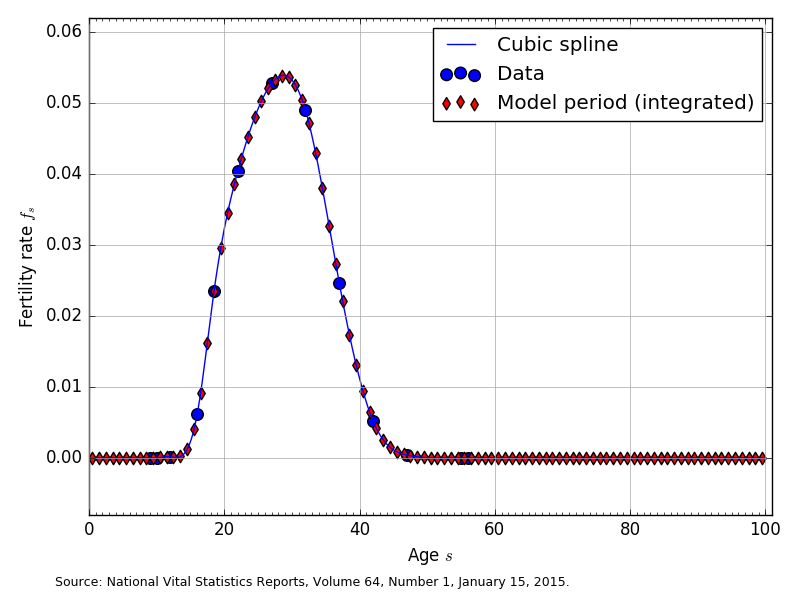
\includegraphics{./images/fert_rates.png}}}
    \end{figure}

    The large blue circles are the 2013 U.S. fertility rate data from \citet{MartinEtAl:2015}. These are 9 fertility rates $[0.3, 12.3, 47.1, 80.7, 105.5, 98.0, 49.3, 10.4, 0.8]$ that correspond to the midpoint ages of the following age (in years) bins $[10-14, 15-17, 18-19, 20-24, 25-29, 30-34, 35-39, 40-44, 45-49]$. In order to get our cubic spline interpolating function to fit better at the endpoints we added to fertility rates of zero to ages 9 and 10, and we added two fertility rates of zero to ages 55 and 56. The blue line in Figure \ref{FigFertRates} shows the cubic spline interpolated function of the data.

    The red diamonds in Figure \ref{FigFertRates} are the average fertility rate in age bins spanning individuals born at the beginning of period 1 (time = 0) and dying at the end of their 100th year. Let the total number of model years that an individual lives be \texttt{totpers}, which is just $E+S\leq 100$. Then the span from 0 to 100 is divided up into \texttt{totpers} bins of equal length. We calculate the average fertility rate in each of the \texttt{totpers} model-period bins as the average population-weighted fertility rate in that span. The red diamonds in Figure \ref{FigFertRates} are the average fertility rates displayed at the midpoint in each of the \texttt{totpers} model-period bins.

    Our fertility rate interpolation function \texttt{get\_fert()} takes as inputs the total number of model periods (\texttt{totpers}) and the range of data year ages that those periods cover. For example, Figure \ref{FigFertRates2} shows the interpolated fertility rates when the total number of periods between age 1 and 100 is 15 periods. Note that there are fewer red diamonds than in Figure \ref{FigFertRates} and that the red diamonds in Figure \ref{FigFertRates2} are just equally spaced out on the interpolated line between 0 and 100. Also note that, because the average fertility rates displayed as red diamonds in Figures \ref{FigFertRates} and \ref{FigFertRates2} are population-weighted averages in each model-period age bin, that the red diamonds do not lie exactly on the cubic spline interpolation (blue line) of fertility rates.

    \begin{figure}[htbp]\centering \captionsetup{width=4.0in}
      \caption{\label{FigFertRates2}\textbf{Fertility rates by age ($f_s$) for $E+S=15$}}
      \fbox{\resizebox{4.0in}{3.0in}{\includegraphics{./images/fert_rates2.png}}}
    \end{figure}


  \subsection{Mortality Rates}\label{AppPopMort}

    The mortality rates in our model $\rho_s$ are a one-period hazard rate and represent the probability of dying within one year, given that an individual is alive at the beginning of period $s$. We assume that the mortality rates for each age cohort $\rho_s$ are constant across time. The infant mortality rate of $\rho_0=0.00587$ comes from the 2015 U.S. CIA World Factbook. Our data for U.S. mortality rates by age come from the Actuarial Life Tables of the U.S. Social Security Administration \citep[see][]{SocSec:2015}, from which the most recent mortality rate data is for 2011. Figure \ref{FigMortRates} shows the mortality rate data and the corresponding model-period mortality rates for $E+S=100$.

    \begin{figure}[htbp]\centering \captionsetup{width=4.0in}
      \caption{\label{FigMortRates}\textbf{Mortality rates by age ($\rho_s$) for $E+S=100$}}
      \fbox{\resizebox{4.0in}{3.0in}{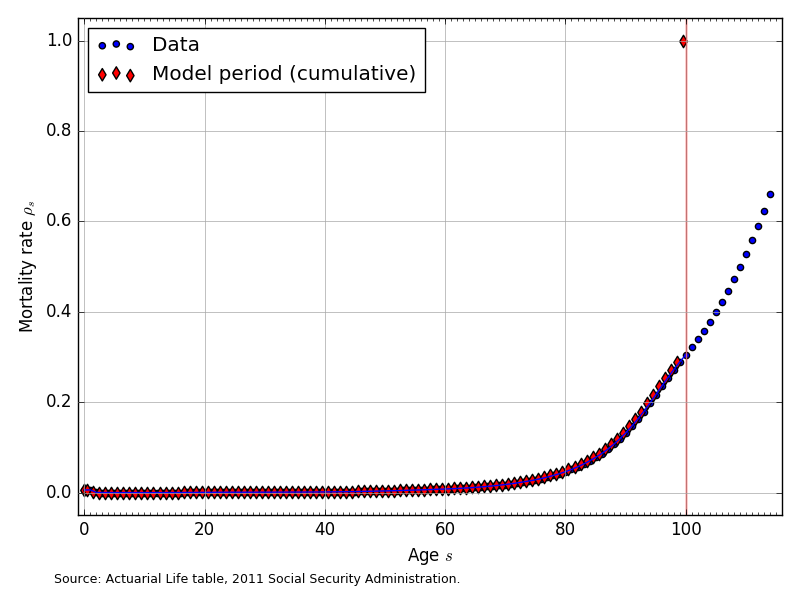
\includegraphics{./images/mort_rates.png}}}
    \end{figure}

    \begin{figure}[htbp]\centering \captionsetup{width=4.0in}
      \caption{\label{FigMortRates2}\textbf{Mortality rates by age ($\rho_s$) for $E+S=15$}}
      \fbox{\resizebox{4.0in}{3.0in}{\includegraphics{./images/mort_rates2.png}}}
    \end{figure}

    The mortality rates in Figure \ref{FigMortRates} are a population-weighted average of the male and female mortality rates reported in \citet{SocSec:2015}. Figure \ref{FigMortRates} also shows that the data provide mortality rates for ages up to 111-years-old. We truncate the maximum age in years in our model to 100-years old. In addition, we constrain the mortality rate to be 1.0 or 100 percent at the maximum age of 100.

    The red diamonds in Figure \ref{FigMortRates} are the interpolated mortality rates for individuals that live for $E+S=100$ periods that range between ages 1 and 100. Our mortality rate interpolation function \texttt{get\_mort()} takes as inputs the total number of periods and the range of data year ages that those periods cover. For example, Figure \ref{FigMortRates2} shows the interpolated mortality rates when the total number of periods between age 1 and 100 is 15 periods. Because mortality rates are cumulative, you will note from in Figure \ref{FigMortRates2} that the mortality rates when model periods are fewer than data periods (the red diamonds) lie strictly above the data mortality rates.\footnote{For example, if two consecutive periods each have a 1 percent mortality rate, then the mortality rate or probability of dying in that two year period is $1-(0.99 \times 0.99) = 0.0199$.}


  \subsection{Immigration Rates}\label{AppPopImm}

    Because of the difficulty in getting accurate immigration rate data by age, we estimate the immigration rates by age in our model $i_s$ as the average residual that reconciles the current-period population distribution with next period's population distribution given fertility rates $f_s$ and mortality rates $\rho_s$. Solving equations \eqref{EqPopLawofmotion} for the immigration rate $i_s$ gives the following characterization of the immigration rates in given population levels in any two consecutive periods $\omega_{s,t}$ and $\omega_{s,t+1}$ and the fertility rates $f_s$ and mortality rates $\rho_s$.

    \begin{equation}\label{EqPopImmRates}
      \begin{split}
        i_1 &= \frac{\omega_{1,t+1} - (1 - \rho_0)\sum_{s=1}^{E+S}f_s\omega_{s,t}}{\omega_{1,t}}\quad\forall t \\
        i_{s+1} &= \frac{\omega_{s+1,t+1} - (1 - \rho_s)\omega_{s,t}}{\omega_{s+1,t}}\qquad\qquad\forall t\quad\text{and}\quad 1\leq s \leq E+S-1
      \end{split}
    \end{equation}

    \begin{figure}[htbp]\centering \captionsetup{width=4.0in}
      \caption{\label{FigImmRates}\textbf{Immigration rates by age ($i_s$), residual, $E+S=100$}}
      \fbox{\resizebox{4.0in}{3.0in}{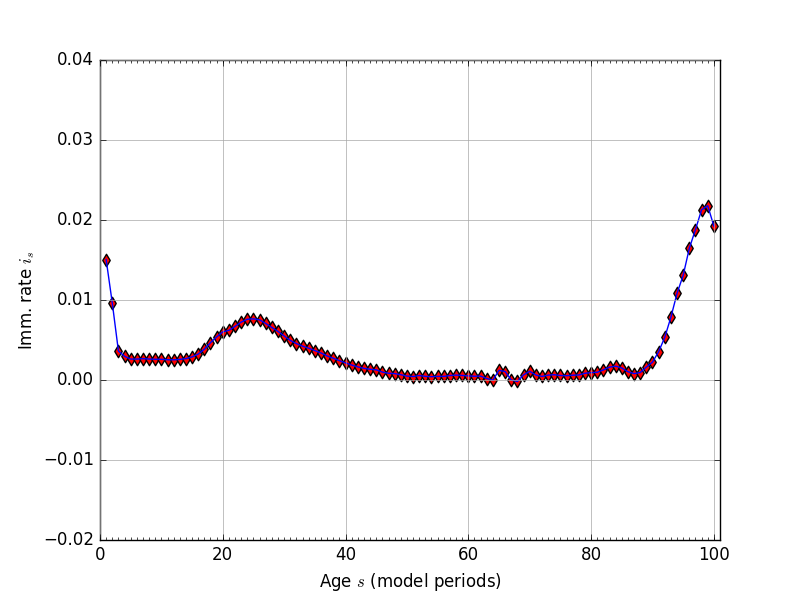
\includegraphics{./images/imm_rates_orig.png}}}
    \end{figure}

    We calculate our immigration rates for three different consecutive-year-periods of population distribution data (2010 through 2013). Our four years of population distribution by age data come from \citet{Census:2015}. The immigration rates $i_s$ that we use in our model are the the residuals described in \eqref{EqPopImmRates} averaged across the three periods. Figure \ref{FigImmRates} shows the estimated immigration rates generated from our \texttt{get\_imm\_resid()} function for $E+S=100$ and given the fertility rates from Section \ref{AppPopFert} and the mortality rates from Section \ref{AppPopMort}.


  \subsection{Population Steady State and Transition}\label{AppPopSStrans}

    This model requires information about mortality rates $\rho_s$ in order to solve for the household's problem each period. It also requires the steady-state stationary population distribution $\bar{\omega}_{s}$ as well as the full transition path of the stationary population distribution $\hat{\omega}_{s,t}$ from the current state to the steady-state. To solve for the steady-state and the transition path of the stationary population distribution, we write the stationary population dynamic equations from \eqref{EqPopLawofmotionStat} in matrix form.
    \begin{equation}\label{EqPopLOMstatmat}
      \begin{split}
        & \begin{bmatrix}
          \hat{\omega}_{1,t+1} \\ \hat{\omega}_{2,t+1} \\ \hat{\omega}_{2,t+1} \\ \vdots \\ \hat{\omega}_{E+S-1,t+1} \\ \hat{\omega}_{E+S,t+1}
        \end{bmatrix}= \frac{1}{1 + g_{n,t+1}} \times ... \\
        & \begin{bmatrix}
          (1-\rho_0)f_1+i_1 & (1-\rho_0)f_2 & (1-\rho_0)f_3 & \hdots & (1-\rho_0)f_{E+S-1} & (1-\rho_0)f_{E+S} \\
          1-\rho_1 & i_2 & 0 & \hdots & 0 & 0 \\
          0 & 1-\rho_2 & i_3 & \hdots & 0 & 0 \\
          \vdots & \vdots & \vdots & \ddots & \vdots & \vdots \\
          0 & 0 & 0 & \hdots & i_{E+S-1} & 0 \\
          0 & 0 & 0 & \hdots & 1-\rho_{E+S-1} & i_{E+S}
        \end{bmatrix}
        \begin{bmatrix}
          \hat{\omega}_{1,t} \\ \hat{\omega}_{2,t} \\ \hat{\omega}_{2,t} \\ \vdots \\ \hat{\omega}_{E+S-1,t} \\ \hat{\omega}_{E+S,t}
        \end{bmatrix}
      \end{split}
    \end{equation}
    We can write system \eqref{EqPopLOMstatmat} more simply in the following way.
    \begin{equation}\label{EqPopLOMstatmat2}
      \bm{\hat{\omega}}_{t+1} = \frac{1}{1+g_{n,t+1}}\bm{\Omega}\bm{\hat{\omega}}_t \quad\forall t
    \end{equation}
    The stationary steady-state population distribution $\bm{\bar{\omega}}$ is the eigenvector $\bm{\omega}$ with eigenvalue $(1+\bar{g}_n)$ of the matrix $\bm{\Omega}$ that satisfies the following version of \eqref{EqPopLOMstatmat2}.
    \begin{equation}\label{EqPopLOMss}
      (1+\bar{g}_n)\bm{\bar{\omega}} = \bm{\Omega}\bm{\bar{\omega}}
    \end{equation}

    \begin{proposition}
      If the age $s=1$ immigration rate is $i_1>-(1-\rho_0)f_1$ and the other immigration rates are strictly positive $i_s>0$ for all $s\geq 2$ such that all elements of $\bm{\Omega}$ are nonnegative, then there exists a unique positive real eigenvector $\bm{\bar{\omega}}$ of the matrix $\bm{\Omega}$, and it is a stable equilibrium.
    \end{proposition}

    \begin{proof}
      First, note that the matrix $\bm{\Omega}$ is square and non-negative.  This is enough for a general version of the Perron-Frobenius Theorem to state that a positive real eigenvector exists with a positive real eigenvalue. This is not yet enough for uniqueness. For it to be unique by a version of the Perron-Fobenius Theorem, we need to know that the matrix is irreducible. This can be easily shown. The matrix is of the form
      $$\bm{\Omega} =
      \begin{bmatrix}
        * & *  & * & \hdots & * & * & *\\
        * & * & 0 & \hdots & 0 & 0 & 0 \\
        0 & * & * & \hdots & 0 & 0 & 0 \\
        \vdots & \vdots & \vdots & \ddots & \vdots & \vdots & \vdots \\
        0 & 0 & 0 & \hdots & *  & * & 0 \\
        0 & 0 & 0 & \hdots & 0 & * & *
      \end{bmatrix}
      $$
      Where each * is strictly positive. It is clear to see that taking powers of the matrix causes the sub-diagonal positive elements to be moved down a row and another row of positive entries is added at the top. None of these go to zero since the elements were all non-negative to begin with.
      $$\bm{\Omega}^2 =
      \begin{bmatrix}
        * & *  & * & \hdots & * & * & *\\
        * & * & * & \hdots & * & * & * \\
        0 & * & * & \hdots & 0 & 0 & 0 \\
        \vdots & \vdots & \vdots & \ddots & \vdots & \vdots & \vdots \\
        0 & 0 & 0 & \hdots & *  & * & 0 \\
        0 & 0 & 0 & \hdots & 0 & * & *
      \end{bmatrix}; ~~~
      \bm{\Omega}^{S+E-1} =
      \begin{bmatrix}
        * & *  & * & \hdots & * & * & *\\
        * & * & * & \hdots & * & * & * \\
        * & * & * & \hdots & * & * & * \\
        \vdots & \vdots & \vdots & \ddots & \vdots & \vdots & \vdots \\
        * & * & * & \hdots & *  & * & * \\
        0 & 0 & 0 & \hdots & 0 & * & *
      \end{bmatrix}
      $$
      $$\bm{\Omega}^{S+E} =
      \begin{bmatrix}
        * & *  & * & \hdots & * & * & *\\
        * & * & * & \hdots & * & * & * \\
        * & * & * & \hdots & * & * & * \\
        \vdots & \vdots & \vdots & \ddots & \vdots & \vdots & \vdots \\
        * & * & * & \hdots & * & * & * \\
        * & * & * & \hdots & * & * & *
      \end{bmatrix}
      $$
      Existence of an $m \in \mathbb N $ such that $\left(\bf\Omega^m\right)_{ij} \neq 0 ~~ ( > 0)$ is one of the definitions of an irreducible (primitive) matrix. It is equivalent to saying that the directed graph associated with the matrix is strongly connected. Now the Perron-Frobenius Theorem for irreducible matrices gives us that the equilibrium vector is unique.

      We also know from that theorem that the eigenvalue associated with the positive real eigenvector will be real and positive. This eigenvalue, $p$, is the Perron eigenvalue and it is the steady state population growth rate of the model. By the PF Theorem for irreducible matrices, $| \lambda_i | \leq p$ for all eigenvalues $\lambda_i$ and there will be exactly $h$ eigenvalues that are equal, where $h$ is the period of the matrix. Since our matrix $\bf\Omega$ is aperiodic, the steady state growth rate is the unique largest eigenvalue in magnitude. This implies that almost all initial vectors will converge to this eigenvector under iteration.
    \end{proof}

    For a full treatment and proof of the Perron-Frobenius Theorem, see \citet{Suzumura:1983}. Because the population growth process is exogenous to the model, we calibrate it to annual age data for age years $s=1$ to $s=100$.

    Figure \ref{FigOrigVsFixSSpop} shows the steady-state population distribution $\bm{\bar{\omega}}$ and the population distribution after 120 periods $\bm{\hat{\omega}}_{120}$. Although the two distributions look very close to each other, they are not exactly the same.

    \begin{figure}[htbp]\centering \captionsetup{width=4.0in}
      \caption{\label{FigOrigVsFixSSpop}\textbf{Theoretical steady-state population distribution vs. population distribution at period $t=120$}}
      \fbox{\resizebox{4.0in}{3.0in}{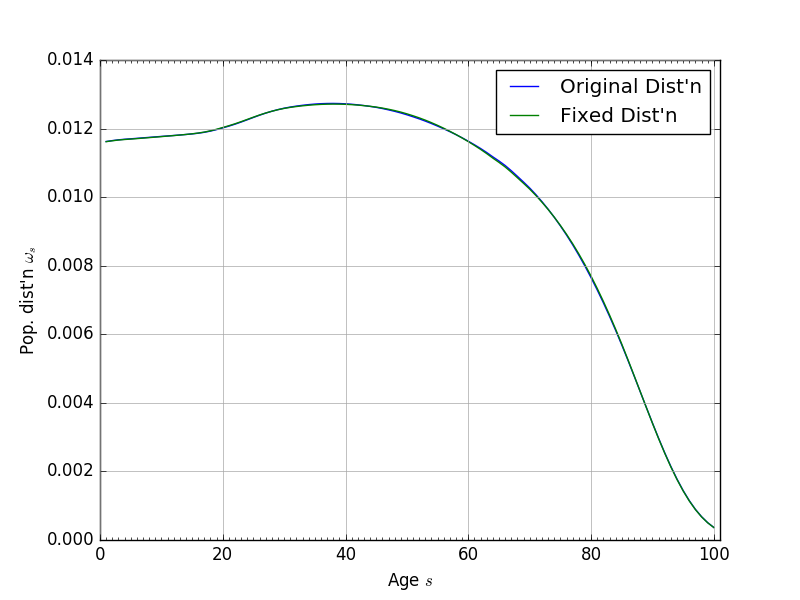
\includegraphics{./images/OrigVsFixSSpop.png}}}
    \end{figure}

    Further, we found that the maximum absolute difference between the population levels $\hat{\omega}_{s,t}$ and $\hat{\omega}_{s,t+1}$ was $1.3852\times 10^{-5}$ after 160 periods. Although this sounds small, the population is still changing after many periods. For equilibrium convergence in our solution method over the transition path of the economy, we need things to be settled down to a steady state after $T$ periods. To do this, we artificially impose that the population distribution in period $t=120$ is the steady-state. As can be seen from Figure \ref{FigOrigVsFixSSpop}, this assumption is not very restrictive. Figure \ref{FigImmRateChg} shows the change in immigration rates that would make the period $t=120$ population distribution equal be the steady-state. This change is not very big. The maximum absolute difference between any two corresponding immigration rates in Figure \ref{FigImmRateChg} is 0.0028.

    \begin{figure}[htbp]\centering \captionsetup{width=4.0in}
      \caption{\label{FigImmRateChg}\textbf{Original immigration rates vs. adjusted immigration rates to make fixed steady-state population distribution}}
      \fbox{\resizebox{4.0in}{3.0in}{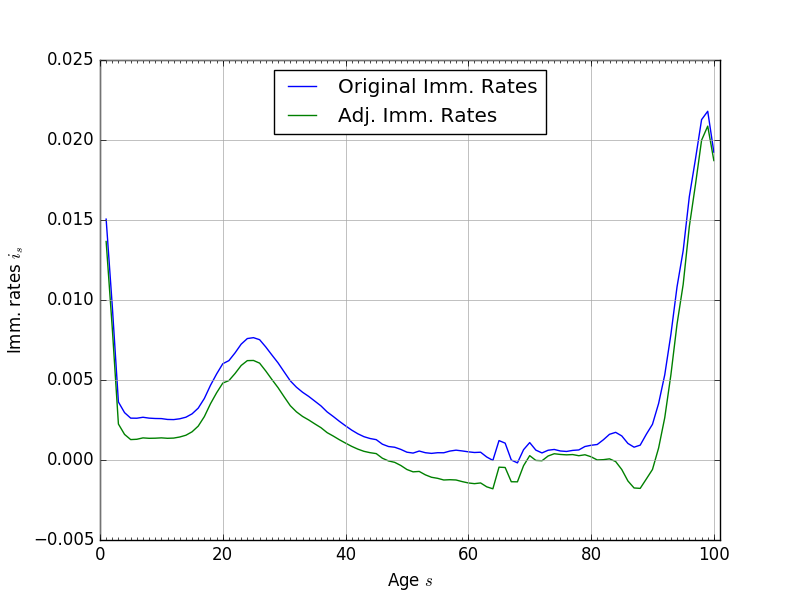
\includegraphics{./images/OrigVsAdjImm.png}}}
    \end{figure}

    The most recent year of population data comes from \citet{Census:2015} population estimates for both sexes for 2013. We those data and use the population transition matrix \eqref{EqPopLOMstatmat2} to age it to the current model year of 2015. We then use \eqref{EqPopLOMstatmat2} to generate the transition path of the population distribution over the time period of the model. Figure \ref{FigPopDistPath} shows the progression from the 2013 population data to the fixed steady-state at period $t=120$. The time path of the growth rate of the economically active population $\tilde{g}_{n,t}$ is shown in Figure \ref{FigGrowthPath}.

    \begin{figure}[htbp]\centering \captionsetup{width=4.0in}
      \caption{\label{FigPopDistPath}\textbf{Stationary population distribution at periods along transition path}}
      \fbox{\resizebox{4.0in}{3.0in}{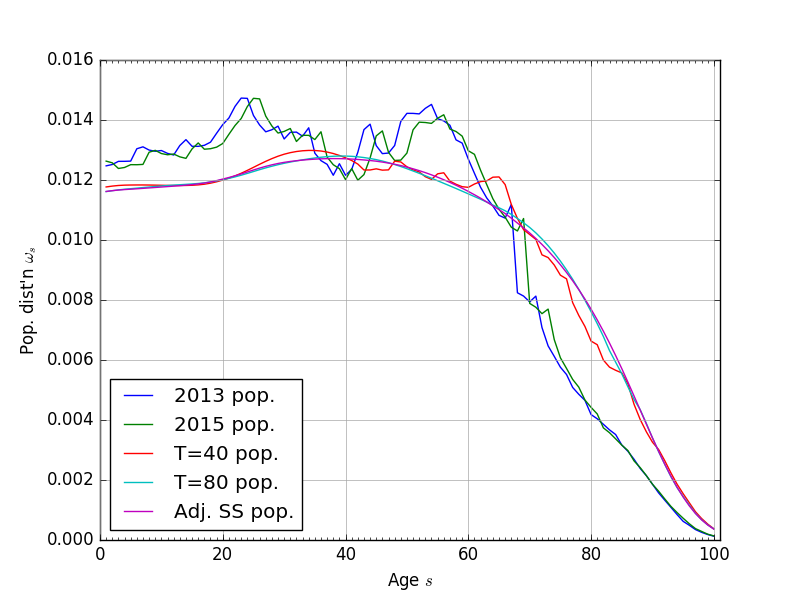
\includegraphics{./images/PopDistPath.png}}}
    \end{figure}

    \begin{figure}[htbp]\centering \captionsetup{width=4.0in}
      \caption{\label{FigGrowthPath}\textbf{Time path of the population growth rate $\tilde{g}_{n,t}$}}
      \fbox{\resizebox{4.0in}{3.0in}{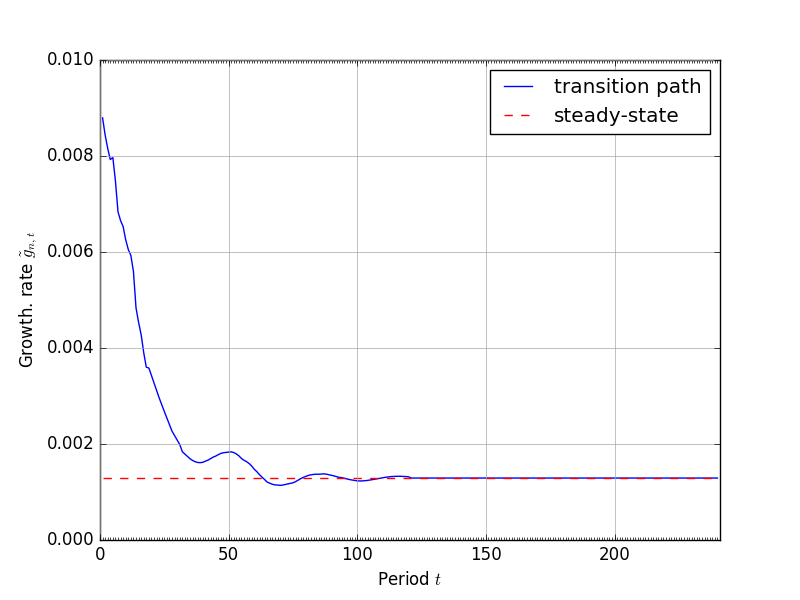
\includegraphics{./images/GrowthPath.png}}}
    \end{figure}
    \clearpage



\newpage
\section{Derivation of elliptical disutility of labor supply}\label{AppEllipseUtil}

  \setcounter{equation}{0}

  \citet{EvansPhillips:2015} provide an exposition of the value of using elliptical disutility of labor specification as well as its relative properties to such standard disutility of labor functions such as constant relative risk aversion (CRRA) and constant Frisch elasticity (CFE). A standard specification of additively separable period utility in consumption and labor supply similar to one used in \citet{KPR:1988} is the following,
  \begin{equation}\label{AppEqStandUtil}
    u(c,n) = \frac{c^{1-\sigma} - 1}{1-\sigma} - \chi^n\frac{\left(n\right)^{1+\theta}}{1+\theta}
  \end{equation}
  where $\sigma\geq 1$ is the coefficient of relative risk aversion on consumption and $\theta\geq 0$ is proportional to the inverse of the Frisch elasticity of labor supply. The constant $\chi^n$ is a scale parameter influencing the relative disutility of labor to the utility of consumption.

  Although labor supply is only defined for $n\in[0,\tilde{l}]$---where $\tilde{l}$ is the time endowment or the maximum labor supply possible---the disutility of labor function in \eqref{AppEqStandUtil} is defined for values of $n$ greater than $\tilde{l}$ and less than 0. Further, for $n<0$, the marginal utility of labor is positive. To avoid the well known and significant computational difficulty of computing the solution to the complementary slackness conditions in the Karush, Kuhn, Tucker constrained optimization problem, we impose an approximating utility function that has properties bounding the solution for $n$ away from both $n=\tilde{l}$ and $n=0$. The upper right quadrant of an ellipse has exactly this property and also has many of the properties of the original utility function. Figure \ref{FigUtilCompar} shows how our estimated elliptical utility function compares to the utility of labor from \eqref{AppEqStandUtil} over the allowed support of $n$.

  \begin{figure}[htb]\centering \captionsetup{width=4.0in}
    \caption{\label{FigUtilCompar}\textbf{Comparison of standard utility of labor $n$ to elliptical utility}}
    \fbox{\resizebox{4.0in}{3.2in}{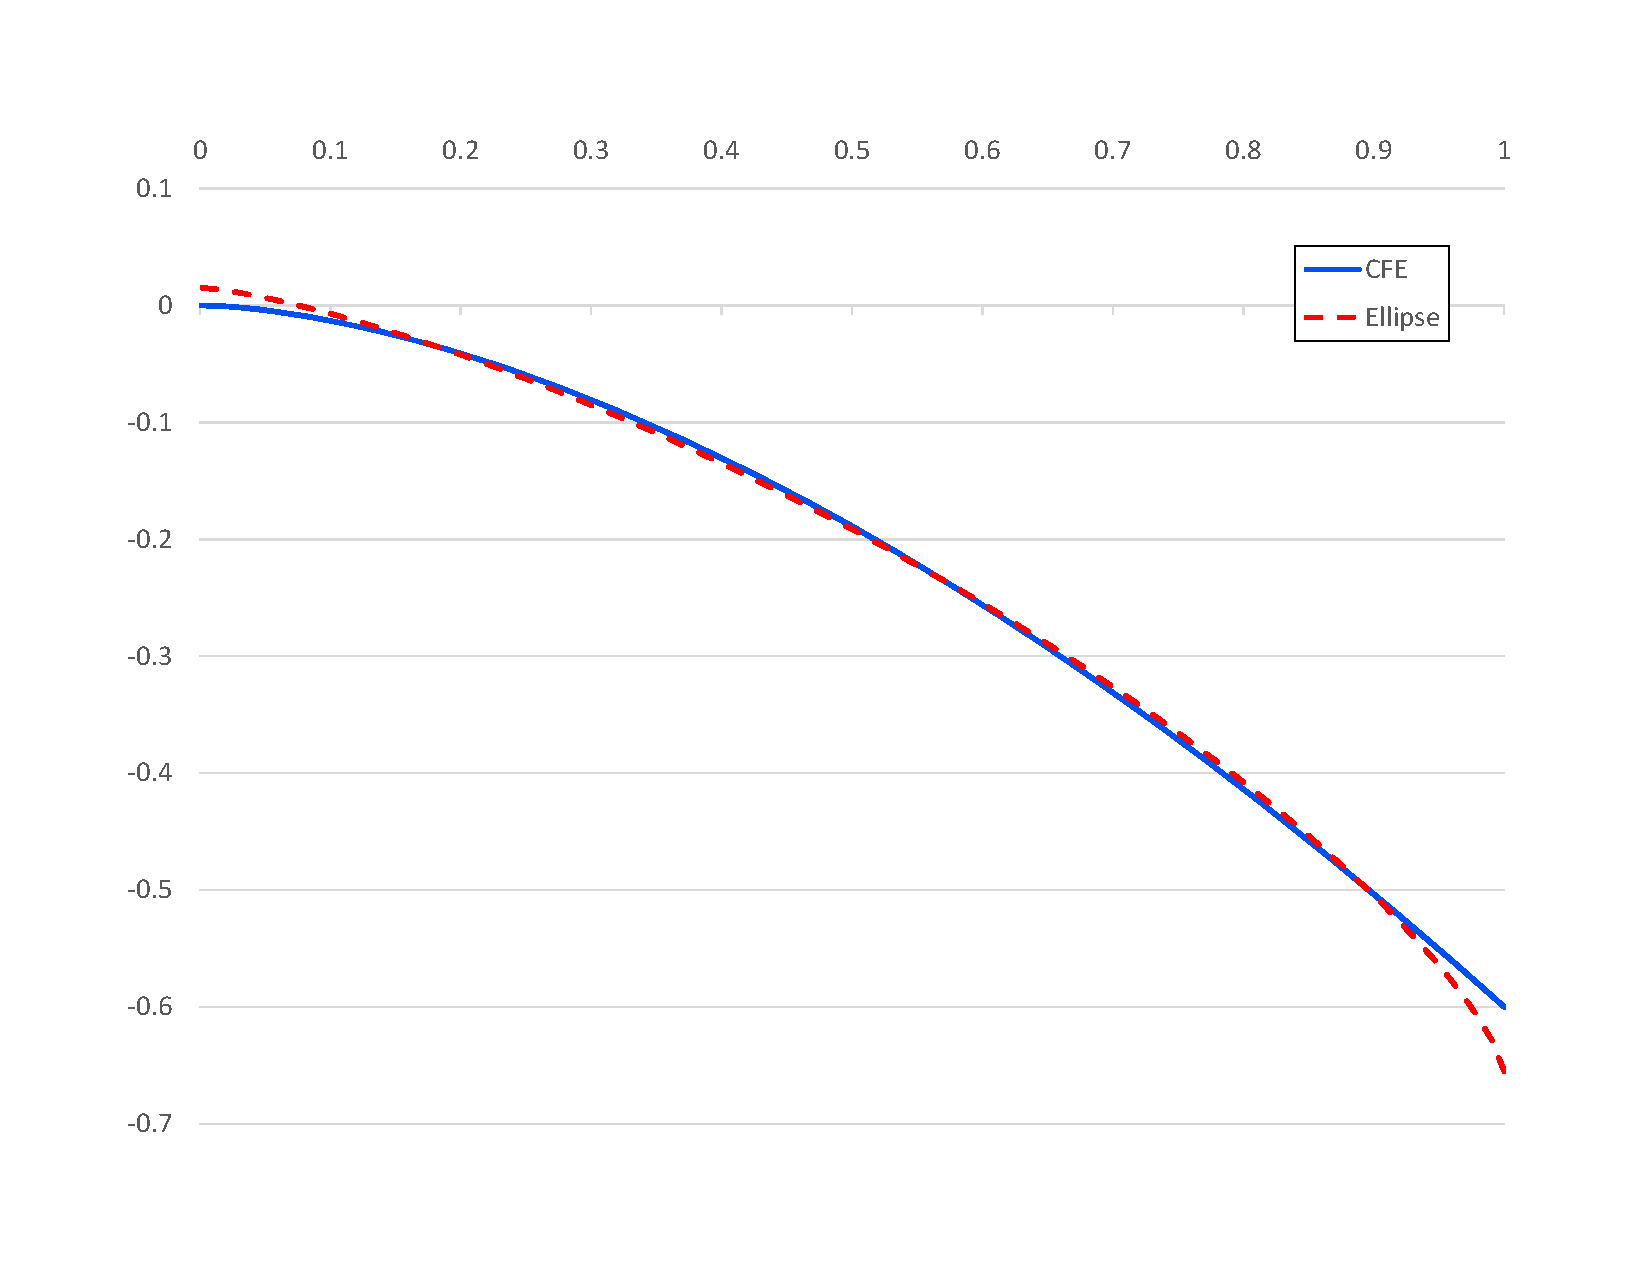
\includegraphics{./images/EllipseUtilComp.pdf}}}
  \end{figure}

  The general equation for an ellipse in $x$ and $y$ space with centroid at coordinates $(h,k)$, horizontal radius of $a$, vertical radius of $b$, and curvature $\upsilon$ is the following.
  \begin{equation}\label{AppEqEllipseGen}
    \left(\frac{x - h}{a}\right)^\upsilon + \left(\frac{y - k}{b}\right)^\upsilon = 1
  \end{equation}
  Figure \ref{FigEllipseGen} shows an ellipse with the parameterization $[h,k,a,b,\upsilon]=[1,-1,1,2,2]$.

  \begin{figure}[htb]\centering \captionsetup{width=3.0in}
    \caption{\label{FigEllipseGen}\textbf{Ellipse with $[h,k,a,b,\upsilon]=[1,-1,1,2,2]$}}
    \fbox{\resizebox{3.0in}{3.8in}{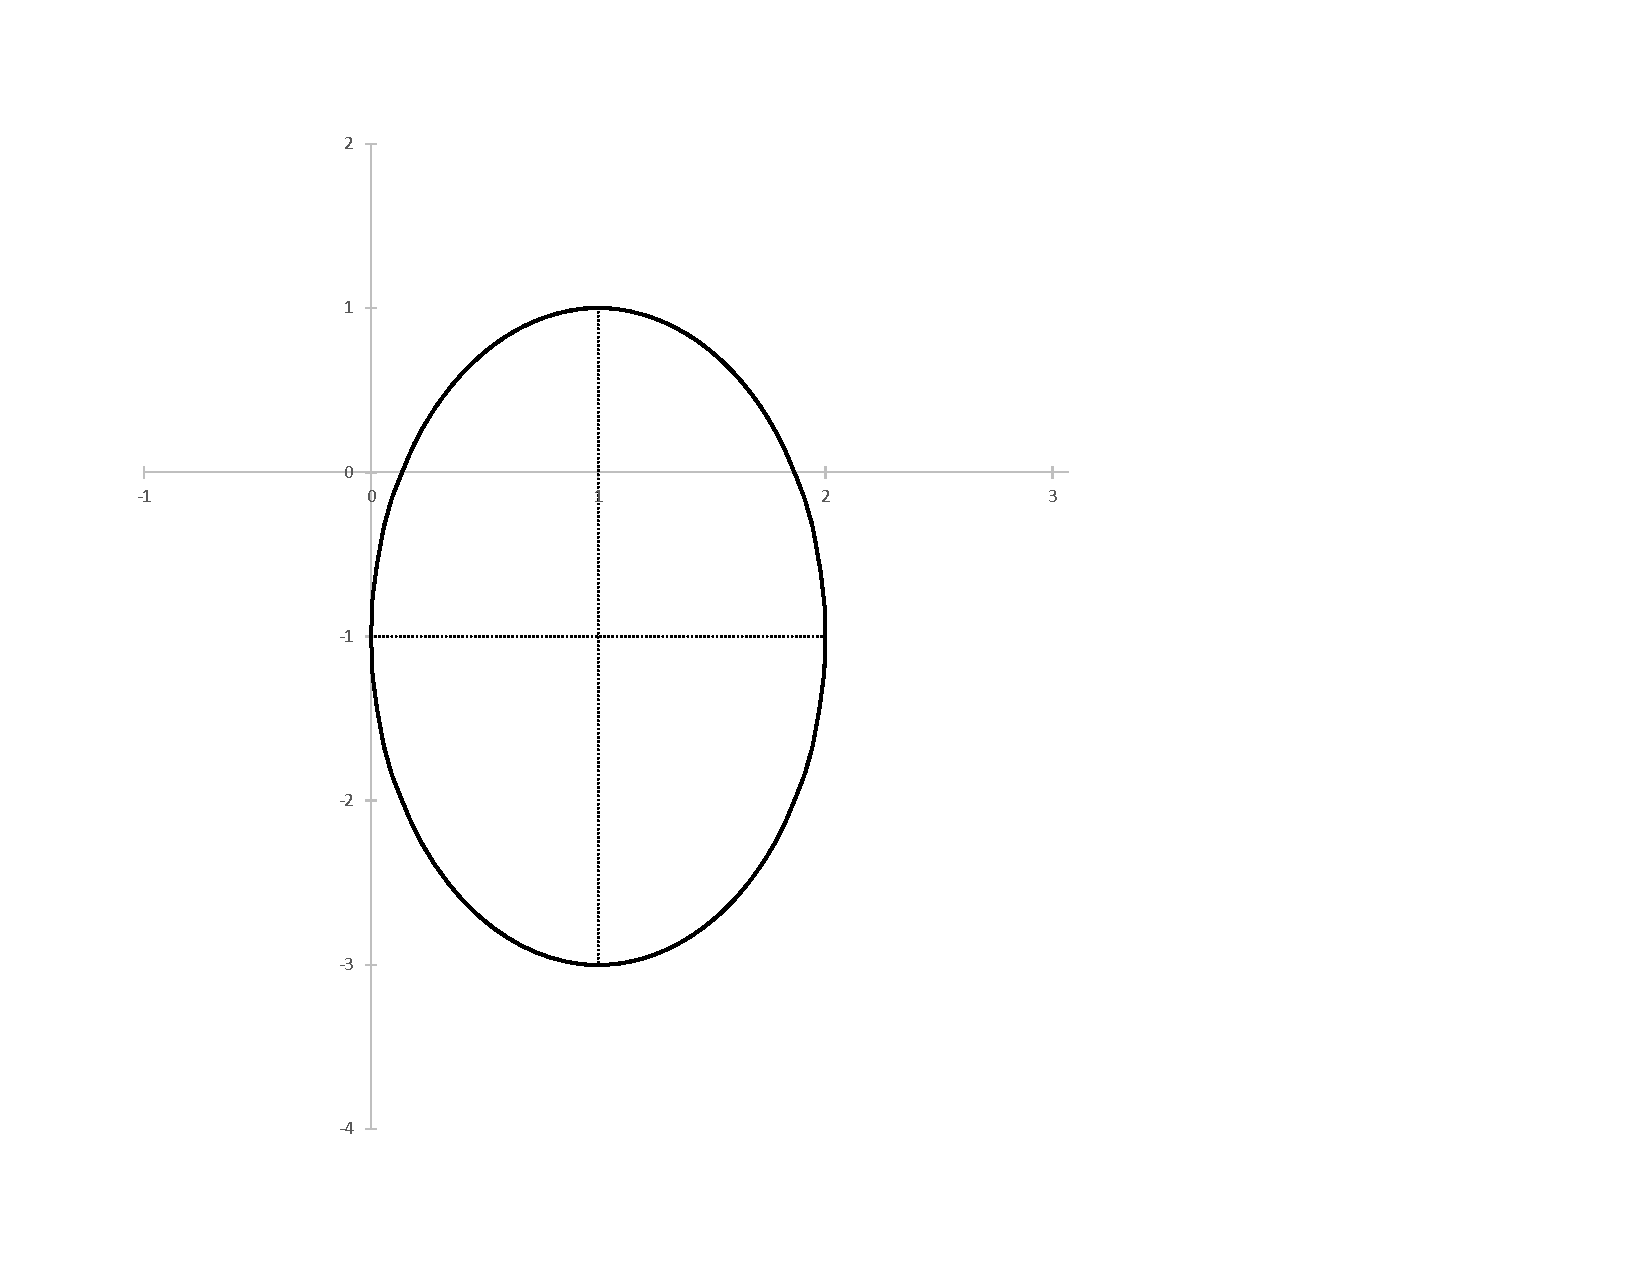
\includegraphics{./images/EllipseGen2.pdf}}}
  \end{figure}

  The graph of the ellipse in the upper-right quadrant of Figure \ref{FigEllipseGen} ($x\in[1,2]$ and $y\in[-1,1]$) has similar properties to the utility of labor term in \eqref{AppEqStandUtil}. If we let the $x$ variable be labor supply $n$, the utility of labor supply be $g(n)$, the $x$-coordinate of the centroid be zero $h=0$, and the horizontal radius of the ellipse be $a=\tilde{l}$, then the equation for the ellipse corresponding to the standard utility specification is the following.
  \begin{equation}\label{AppEqEllipseN}
    \left(\frac{n}{\tilde{l}}\right)^\upsilon + \left(\frac{g - k}{b}\right)^\upsilon = 1
  \end{equation}
  Solving the equation for $g$ as a function of $n$, we get the following.
  \begin{equation}\label{AppEqGn}
    g(n) = b\left[1 - \left(\frac{n}{\tilde{l}}\right)^\upsilon\right]^{\frac{1}{\upsilon}} + k
  \end{equation}
  The $\upsilon$ parameter acts like a constant elasticity of substitution, and the parameter $b$ is a shape parameter similar to $\chi^n$ in \eqref{AppEqStandUtil}.

  We use the upper-right quadrant of the elliptical utility function because the utility of $n$ is strictly decreasing on $n\in(0,\tilde{l})$, because the slope of the utility function goes to negative infinity as $n$ approaches its maximum of $\tilde{l}$ and because the slope of the utility function goes to zero as $n$ approaches its minimum of 0. This creates interior solutions for all optimal labor supply choices $n^*\in(0,\tilde{l})$. Although it is more realistic to allow optimal labor supply to sometimes be zero, the complexity and dimensionality of our model requires this approximating assumption to render the solution method tractable.

  Figure \ref{FigUtilCompar} shows how closely the estimated elliptical utility function matches the original utility of labor function in \eqref{AppEqStandUtil} with a Frisch elasticity of 0.4.\footnote{See \citet{Chetty:2011}, \citet{KeaneRogerson:2012} and \citet{Peterman:2014} for discussion of this choice.} We choose the ellipse parameters $b$, $k$, and $\upsilon$ to best match the points on the original utility of labor function for $n\in[0,0.9]$. We minimize the sum of absolute errors for 101 evenly spaced points on this domain. The estimated values of the parameters for the elliptical utility shown in Figure \ref{FigUtilCompar} and represented in equation \eqref{AppEqGn} are $[b,k,\upsilon] = [0.573,0.000,2.856]$.

  \clearpage


\newpage
\section{Solving for stationary steady-state equilibrium}\label{AppSSsolve}

  \setcounter{equation}{0}
  \renewcommand\theenumi{\arabic{enumi}}
  \renewcommand\theenumii{\alph{enumii}}
  \renewcommand\theenumiii{\roman{enumiii}}

  This section describes the solution method for the stationary steady-state equilibrium described in Definition \ref{DefEquilSS}. The steady-state is characterized by $2JS$ equations and $2JS$ unknowns. However, because some of the other equations cannot be solved for analytically and substituted into the Euler equations, we must take a two-stage approach to the equilibrium solution. We first make a guess at steady-state wage $\bar{w}$, interest rate $\bar{r}$, lump-sum transfer $\bar{T}^H$, and income multiplier $factor$. Then, given those four aggregate variables, we can solve for the second-stage household decisions of steady-state savings $\bar{b}_{j,s}$ and labor supply $\bar{n}_{j,s}$.

  \begin{enumerate}
    \item Use the techniques in Appendix \ref{AppPopDyn} to solve for the steady-state population distribution vector $\bm{\bar{\omega}}$ of the exogenous population process.
    \item Choose an initial guess for the values of the steady-state wage $\bar{w}$, interest rate $\bar{r}$, lump-sum transfer $\bar{T}^H$, and income multiplier $factor$.
    \item Given guesses for $\bar{w}$, $\bar{r}$, $\bar{T}^H$, and $factor$, solve for the steady-state household savings $\bar{b}_{j,s}$ and labor supply $\bar{n}_{j,s}$ decisions using $2JS$ equations \eqref{EqEulerLabStat}, \eqref{EqEulerSavStat}.
      \begin{itemize}
        \item A good first guess for $\bar{b}_{j,s}$ and $\bar{n}_{j,s}$ is a number close to but less than $\tilde{l}$ for all the $\bar{n}_{j,s}$ and to choose some small positive number for $\bar{b}_{j,s}$ that is small enough to be less than the minimum income that an individual might have $\bar{w}e_{j,s}\bar{n}_{j,s}$.
        \item Make sure that all of the $2JS$ Euler errors is sufficiently close to zero to constitute a solution.
      \end{itemize}
    \item Given the solutions $\bar{b}_{j,s}$ and $\bar{n}_{j,s}$ from step (3), make sure that the four characterizing equations for $\bar{w}$, $\bar{r}$, $\bar{T}^H$, and $factor$ are solved. These characterizing equations are the zero equations corresponding to the steady-state versions of \eqref{EqFOCwageStat}, \eqref{EqFOCrate}, \eqref{EqGovtBCstat}, and \eqref{EqIncFactor}.
      \begin{align}
        \bar{w} - (1-\alpha)\frac{\bar{Y}}{\bar{L}} &= 0 \label{EqFOCwageSS0} \\
        \bar{r} - \alpha\frac{\bar{Y}}{\bar{K}} + \delta &= 0 \label{EqFOCrateSS0} \\
        \bar{T}^H - \sum_s \sum_j \bar{\omega}_s\lambda_j \bar{T}_{s} &= 0 \label{EqGovtBCSS0} \\
        factor\sum_s \sum_j \bar{\omega}_s\lambda_j\left(\bar{w}e_{j,s}\bar{n}_{j,s} + \bar{r}\bar{b}_{j,s}\right) - \left(\text{data avg. income}\right) &= 0 \label{EqIncFactorSS0}
      \end{align}
    \item Iterate on guesses for outer loop values of $\bar{w}$, $\bar{r}$, $\bar{T}^H$, and $factor$ until the Euler equations from step (3) and the characterizing equations from step (4) are all solved.
  \end{enumerate}


\newpage
\section{Solving for stationary non-steady-state equilibrium by time path iteration}\label{AppNonSSsolve}

  \setcounter{equation}{0}

  This section describes the solution to the non-steady-state transition path equilibrium of the model described in Definition \ref{DefEquilNonSS} and outlines the time path iteration (TPI) method of \citet{AuerbachKotlikoff:1987} for solving for this equilibrium. The following are the steps for computing a stationary non-steady-state equilibrium time path for the economy.
  \begin{enumerate}
    \item Input all initial parameters. See Table \ref{TabExogVars}.
      \begin{enumerate}
        \item The value for $T$ at which the non-steady-state transition path should have converged to the steady state should be at least as large as the number of periods it takes the population to reach its steady state $\bm{\bar{\omega}}$ as described in Appendix \ref{AppPopDyn}.
      \end{enumerate}
    \item Choose an initial distribution of savings and intended bequests $\bm{\hat{\Gamma}}_1$ and then calculate the initial state of the stationarized aggregate capital stock $\hat{K}_1$ and total bequests received $\hat{BQ}_{j,1}$ consistent with $\bm{\hat{\Gamma}}_1$ according to \eqref{EqMktClrCapStat} and \eqref{EqTotBeqStat}.
      \begin{enumerate}
        \item Note that you must have the population weights from the previous period $\hat{\omega}_{s,0}$ and the growth rate between period 0 and period 1 $\tilde{g}_{n,1}$ to calculate $\hat{BQ}_{j,1}$.
      \end{enumerate}
    \item Conjecture transition paths for the stationarized wage $\bm{\hat{w}}^1=\{\hat{w}^1_t\}_{t=1}^\infty$, stationarized interest rate $\bm{r}^1=\{r^1_t\}_{t=1}^\infty$, total bequests received $\bm{\hat{BQ}}_j^1=\{\hat{BQ}^{1}_{j,t}\}_{t=1}^\infty$ for each household type $j$, and the lump-sum transfer from the government $\bm{\hat{T}^{H,1}}=\{\hat{T}^{H,1}_t\}_{t=1}^\infty$. The only requirements are that $\hat{K}^i_1$ and $\hat{BQ}^i_{j,1}$ are functions of the initial distribution of savings $\bm{\hat{\Gamma}}_1$ for all iterations $i$ in your initial state and that the time paths of $\bm{\hat{w}}^i$, $\bm{r}^i$, $\bm{\hat{BQ}}_j^i$, and $\bm{\hat{T}^{H,i}}$ equal their respective steady-state values for all $t\geq T$.
      \begin{enumerate}
        \item Initial guesses for $\hat{w}_1$ and $r_1$ can be disciplined a little bit by whether $\hat{K}_1$ is greater than or less than $\bar{K}$. If $\hat{K}_1 > \bar{K}$, then choose $\hat{w}_1 > \bar{w}$ and $r_1 < \bar{r}$. If $\hat{K}_1 < \bar{K}$, then choose $\hat{w}_1 < \bar{w}$ and $r_1 > \bar{r}$.
      \end{enumerate}
    \item With the conjectured transition paths $\bm{\hat{w}}^i$, $\bm{r}^i$, $\bm{\hat{BQ}}_j^i$, and $\bm{\hat{T}^{H,i}}$, one can solve for the lifetime labor and savings decisions for each individual in the model who will be alive between periods $t=1$ and $T$. Each individual's lifetime decisions can be solved independently using the systems of $2S$ Euler equations of the form \eqref{EqEulerLabStat}, \eqref{EqEulerSavStat}, and \eqref{EqEulerSavEpSstat}.
      \begin{enumerate}
        \item Make sure all the Euler errors for both the savings and labor supply decisions are sufficiently close to zero in order to ensure that the household equilibrium is being solved.
      \end{enumerate}
    \item Use the implied distribution of savings and labor supply in each period to compute the new implied time paths for the wage $\bm{\hat{w}}^{i'} = \{\hat{w}_1^i,\hat{w}_2^{i'},...\hat{w}_T^{i'}\}$, interest rate $\bm{r}^{i'} = \{r_1^i,r_2^{i'},...r_T^{i'}\}$, total bequests received $\bm{\hat{BQ}}_j^{i'} = \{\hat{BQ}_{j,1}^i,\hat{BQ}_{j,2}^{i'},...\hat{BQ}_{j,T}^{i'}\}$ for each ability group $j$, and lump-sum transfer from the government $\bm{\hat{T}^{H,i'}} = \{\hat{T}_1^{H,i'},\hat{T}_2^{H,i'},...\hat{T}_T^{H,i'}\}$.
    \item Check the distance between the two sets time paths.
      \begin{equation*}
        \norm{\Bigl[\bm{\hat{w}}^{i'}, \bm{r}^{i'},\bigl\{\bm{\hat{BQ}}_j^{i'}\bigr\}_{j=1}^J, \bm{\hat{T}^{H,i'}}\Bigr] - \Bigl[\bm{\hat{w}}^{i}, \bm{r}^{i},\bigl\{\bm{\hat{BQ}}_j^{i}\bigr\}_{j=1}^J, \bm{\hat{T}^{H,i}}\Bigr]}
      \end{equation*}
      \begin{enumerate}
        \item If the distance between the initial time paths and the implied time paths is less-than-or-equal-to some convergence criterion $\ve>0$, then the fixed point has been achieved and the equilibrium time path has been found.
        \item If the distance between the initial time paths and the implied time paths is greater than some convergence criterion $\norm{\cdot}>\ve$, then update the guess for the time paths and repeat steps (4) through (6) until a fixed point is reached.
      \end{enumerate}
  \end{enumerate}

  Figures \ref{FigKpathTPI} and \ref{FigLpathTPI} show the equilibrium time paths of the aggregate capital stock $K_t$ and aggregate labor supply $L_t$ for the calibration of the model in this paper.

  \begin{figure}[htb]\centering \captionsetup{width=4.0in}
    \caption{\label{FigKpathTPI}\textbf{Equilibrium time path of $K_t$ for $S=80$ and $J=7$ in baseline model}}
    \fbox{\resizebox{4.0in}{3.0in}{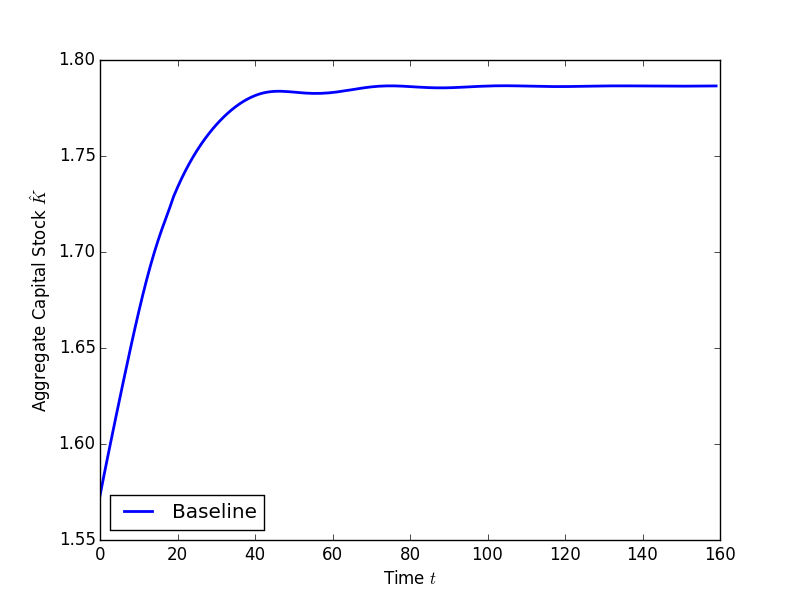
\includegraphics{./images/TPI_K.png}}}
  \end{figure}

  \begin{figure}[htb]\centering \captionsetup{width=4.0in}
    \caption{\label{FigLpathTPI}\textbf{Equilibrium time path of $L_t$ for $S=80$ and $J=7$ in baseline model}}
    \fbox{\resizebox{4.0in}{3.0in}{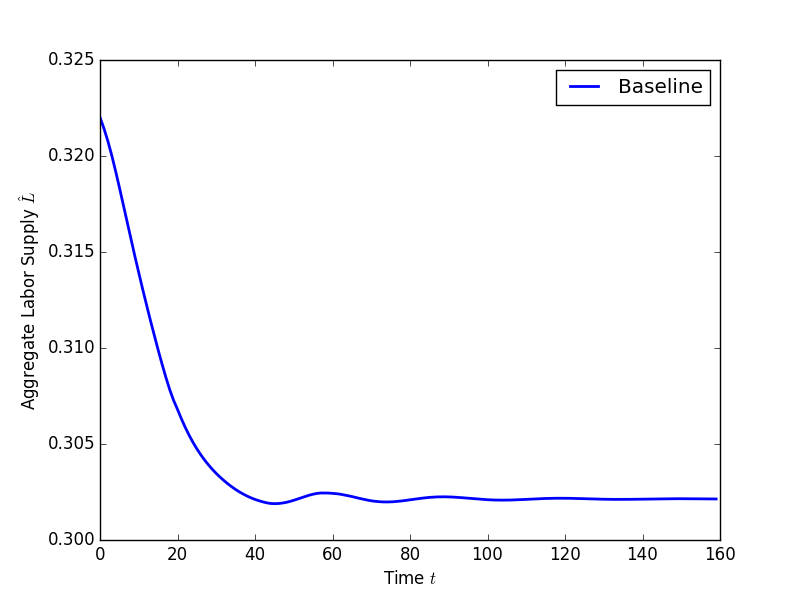
\includegraphics{./images/TPI_L.png}}}
  \end{figure}

  \clearpage


\end{document}
